% Informe del proyecto de generación de código intermedio (TAC) de Compiscript.
% Compilar con: tectonic -X compile informe.tex
\documentclass[11pt,a4paper]{article}

\usepackage[T1]{fontenc}
\usepackage{lmodern}
\usepackage[spanish,es-tabla,es-noquoting]{babel}
\usepackage[margin=2.5cm]{geometry}
\usepackage{graphicx}
\usepackage{xcolor}
\usepackage{booktabs}
\usepackage{longtable}
\usepackage{array}
\usepackage{tabularx}
\usepackage{listings}
\usepackage{caption}
\usepackage{float}
\usepackage{enumitem}
\usepackage{fancyhdr}
\usepackage{needspace}
\usepackage[hidelinks]{hyperref}

\definecolor{fondoCodigo}{RGB}{247,248,250}
\definecolor{bordeCodigo}{RGB}{200,205,214}
\definecolor{comentario}{RGB}{95,120,95}
\definecolor{palabraClave}{RGB}{40,70,150}
\definecolor{cadena}{RGB}{150,60,40}
\definecolor{etiquetaTAC}{RGB}{120,50,120}
\definecolor{verdeUVG}{RGB}{0,105,60}

\lstdefinelanguage{Compiscript}{
  morekeywords={let,const,var,function,class,new,this,return,if,else,while,
    do,for,foreach,in,break,continue,switch,case,default,try,catch,print,
    integer,float,string,boolean,void,null,true,false},
  sensitive=true,
  morecomment=[l]{//},
  morecomment=[s]{/*}{*/},
  morestring=[b]",
}

% Lenguaje intermedio TAC de Compiscript: palabras de control resaltadas.
\lstdefinelanguage{TAC}{
  morekeywords={begin_program,end_program,class,endclass,field,func,endfunc,
    param_in,param,call,call_method,return,declare,goto,if,ifFalse,capture,
    static_link,newlist,new,length,print,try_begin,catch,try_end,extends,from},
  sensitive=true,
  morecomment=[l]{//},
  morestring=[b]",
}

\lstset{
  basicstyle=\ttfamily\footnotesize,
  keywordstyle=\color{palabraClave}\bfseries,
  commentstyle=\color{comentario},
  stringstyle=\color{cadena},
  backgroundcolor=\color{fondoCodigo},
  frame=single,
  rulecolor=\color{bordeCodigo},
  breaklines=true,
  showstringspaces=false,
  extendedchars=true,
  numbers=left,
  numberstyle=\tiny\color{gray},
  numbersep=8pt,
  xleftmargin=18pt,
  framexleftmargin=18pt,
  captionpos=b,
}

% Listado sin numeración para los fragmentos pequeños de TAC.
\lstdefinestyle{sinnumero}{numbers=none,xleftmargin=4pt,framexleftmargin=4pt}

\pagestyle{fancy}
\fancyhf{}
\fancyhead[L]{\small Fase de Compilación: Generación de Código Intermedio}
\fancyhead[R]{\small Compiscript --- ANTLR + C++}
\fancyfoot[C]{\thepage}
\renewcommand{\headrulewidth}{0.4pt}

\captionsetup{font=small,labelfont=bf}
\setlength{\parskip}{0.5em}
\setlength{\parindent}{0pt}

\newcolumntype{L}[1]{>{\raggedright\arraybackslash}p{#1}}

% Encabezado en línea propia para las tablas que siguen (un \paragraph en línea
% quedaría después del flotante).
\newcommand{\subhead}[1]{\par\medskip\noindent\textbf{#1}\par\nopagebreak\smallskip}

\begin{document}

% ------------------------------------------------------------------ CARÁTULA
\begin{titlepage}
\begin{center}

\vspace*{0.2cm}


\includegraphics[width=0.24\textwidth]{img/uvg-logo.png}

\vspace{0.8cm}

{\Large\scshape Universidad del Valle de Guatemala}\\[0.30cm]
{\large Facultad de Ingeniería}\\[0.20cm]
{\large Departamento de Ciencias de la Computación}\\[0.20cm]
{\large Construcción de Compiladores}

\vspace{1.1cm}

\rule{\textwidth}{0.8pt}

\vspace{0.5cm}

{\Huge\bfseries [M2] Fase de Compilación:}\\[0.30cm]
{\Huge\bfseries Generación de Código Intermedio}

\vspace{0.5cm}

{\Large Generador de código de tres direcciones de Compiscript}\\[0.30cm]
{\small ANTLR 4.13.2 \ $\bullet$ \ C++17 \ $\bullet$ \ TAC \ $\bullet$ \ IDE web}\\[0.30cm]
{\scriptsize\url{https://github.com/G1LB3T0/Proyecto1_Compis_Generador_Analizador_Lexico/tree/Compiladores2-Proyecto2}}

\vspace{0.5cm}

\rule{\textwidth}{0.8pt}

\vspace{1.2cm}

{\large\bfseries Catedrático}\\[0.25cm]
{\large Ing. Pablo Koch}

\vspace{0.9cm}

{\large\bfseries Integrantes}\\[0.3cm]
{\large Luis Gonzalez --- 23353}\\[0.2cm]
{\large Joel Jaquez --- 23369}

\vfill

{\large Guatemala, 18 de octubre de 2026}

\end{center}
\end{titlepage}

\tableofcontents
\newpage

% ------------------------------------------------------------ 1 INTRODUCCIÓN
\section{Introducción}

Este informe documenta la fase de \textbf{generación de código intermedio} del
compilador de \textbf{Compiscript}, un lenguaje basado en un subconjunto de
TypeScript. El trabajo parte de lo construido en la fase anterior ---el
analizador sintáctico y semántico con su tabla de símbolos--- y agrega una
segunda pasada que recorre el mismo árbol sintáctico y lo traduce a
\textbf{código de tres direcciones} (TAC, por \emph{three-address code}), la
representación que servirá de base para una posterior generación de código
ensamblador u objeto.

Como en la fase anterior, \textbf{todo el compilador está escrito en C++17}.
El generador de código es un segundo \emph{Visitor} de ANTLR, el
\texttt{TacGenerator}, que se enlaza en la misma biblioteca nativa que el
analizador semántico. Python aparece únicamente como adaptador web (el servidor
Flask que sirve el IDE) y JavaScript únicamente para presentar resultados:
ninguna regla de traducción está implementada fuera de C++.

La fase aporta tres piezas, que corresponden a los componentes evaluados:

\begin{itemize}[leftmargin=1.4em]
  \item \textbf{Un lenguaje intermedio documentado}: cuádruplos con operación,
        dos argumentos y un resultado, con una forma textual legible y un
        conjunto de instrucciones para datos, control de flujo, funciones,
        closures, clases y listas.
  \item \textbf{Un generador de TAC} que traduce expresiones, declaraciones,
        \texttt{if/else}, \texttt{while}, \texttt{do-while}, \texttt{for},
        \texttt{foreach}, \texttt{switch}, \texttt{break}, \texttt{continue},
        funciones recursivas y anidadas, clases, objetos y listas, con un
        algoritmo de asignación y reciclaje de variables temporales.
  \item \textbf{Una tabla de símbolos extendida} con tamaños, desplazamientos,
        clase de almacenamiento, etiquetas y profundidad léxica, más el diseño
        abstracto de los \textbf{registros de activación} de cada función.
\end{itemize}

El sistema acepta archivos \texttt{.cps} y produce, en un único documento JSON,
los tokens, el árbol sintáctico, los diagnósticos, la tabla de símbolos con la
información de generación de código, el texto TAC, los cuádruplos y los
registros de activación. La batería de pruebas pasa de 95 a \textbf{107
escenarios} y todos aprueban.

% -------------------------------------------------------------- 2 OBJETIVOS
\section{Objetivos}

\subsection{Objetivo general}

Implementar un generador de código intermedio para Compiscript que, a partir
del árbol sintáctico y la tabla de símbolos producidos por el análisis
semántico, emita código de tres direcciones correcto y documentado, manejando
temporales, entornos de ejecución y registros de activación.

\subsection{Objetivos específicos}

\begin{itemize}[leftmargin=1.4em]
  \item Diseñar y documentar un lenguaje intermedio de tres direcciones, con
        sintaxis consistente y ejemplos de traducción.
  \item Traducir expresiones aritméticas, lógicas y de comparación respetando
        precedencia y asociatividad, y las declaraciones y asignaciones de
        variables y constantes.
  \item Traducir el control de flujo (\texttt{if/else}, \texttt{while},
        \texttt{do-while}, \texttt{for}, \texttt{foreach}, \texttt{switch},
        \texttt{break} y \texttt{continue}) mediante etiquetas y saltos.
  \item Traducir funciones, paso de parámetros, retorno, recursividad, funciones
        anidadas y closures, así como clases, objetos, métodos, atributos y
        listas.
  \item Implementar un algoritmo de asignación y reciclaje de temporales que
        minimice la cantidad de temporales vivos.
  \item Extender la tabla de símbolos con direcciones, desplazamientos, tamaños
        y etiquetas, y modelar registros de activación.
  \item Ampliar la batería de pruebas y el IDE para ejecutar y mostrar la
        generación de código intermedio.
\end{itemize}

% ------------------------------------------------------------ 3 ARQUITECTURA
\section{Arquitectura general}

\subsection{El pipeline}

El flujo de información va del texto fuente al documento JSON que consume el
IDE. Cada etapa tiene una responsabilidad única y un artefacto observable. Las
dos etapas nuevas de esta fase son el \texttt{TacGenerator} y la extensión de la
tabla de símbolos:

\begin{center}
\begin{minipage}{0.86\textwidth}
\ttfamily\small
\begin{verbatim}
Código .cps
    |
    v
CompiscriptLexer  (ANTLR, C++)
    | tokens
    v
CompiscriptParser (ANTLR, C++)
    | parse tree ---------> tree_serializer -> árbol JSON -> IDE
    v
SemanticAnalyzer  (Visitor C++, primera pasada)
    |-- tipos, ámbitos, funciones, clases, listas
    |-- tabla de símbolos + SemanticBindings
    v
(solo si no hay errores léxicos, sintácticos ni semánticos)
    v
TacGenerator      (Visitor C++, segunda pasada)  <<< NUEVO
    |-- layoutSymbols: tamaños, offsets, etiquetas, frames
    |-- traducción a cuádruplos con pool de temporales
    v
JSON: diagnósticos + símbolos + TAC + registros de activación
    |
    v
Flask (adaptador) -> IDE web (pestaña "Código TAC")
\end{verbatim}
\end{minipage}
\end{center}

\subsection{Dos Visitors con responsabilidades distintas}

\texttt{SemanticAnalyzer} y \texttt{TacGenerator} son Visitors diferentes. El
primero decide qué significa cada identificador, comprueba tipos y construye los
ámbitos. El segundo consume esa información y vuelve a recorrer el mismo árbol
para emitir instrucciones. Separarlos evita duplicar la resolución de nombres y
garantiza que el generador nunca intente corregir ni reinterpretar un programa
inválido.

El puente entre ambos es la estructura \texttt{SemanticBindings}, que el
analizador llena mientras recorre el árbol. Asocia cada nodo del
\emph{parse tree} con tres cosas:

\begin{itemize}[leftmargin=1.4em]
  \item \texttt{symbols}: el identificador del símbolo al que se refiere un
        nodo (una declaración, un uso, una llamada, un \texttt{new});
  \item \texttt{scopes}: el ámbito que abre un nodo (programa, bloque, función,
        clase, \texttt{for}, \texttt{foreach}, \texttt{catch});
  \item \texttt{expressions}: el tipo sintetizado de cada expresión.
\end{itemize}

Estas asociaciones son efímeras: viven solo mientras \texttt{analyzeSource}
conserva el árbol de ANTLR. Gracias a ellas el generador no resuelve nombres
por texto, sino por identificador de símbolo; el sufijo \texttt{\#id} que
aparece en el TAC (por ejemplo \texttt{@x\#2}) es ese identificador, y es lo que
evita que dos variables sombreadas compartan una misma dirección.

\subsection{Núcleo independiente de la interfaz}

El núcleo C++ sigue exponiendo una sola función pública, \texttt{analyzeSource},
que devuelve un \texttt{AnalysisResult}. El CLI, la batería de pruebas y el
servidor Flask la usan por igual, de modo que lo que prueba la batería es
exactamente lo que ejecuta el IDE. El resultado ahora incluye el \texttt{tac}
(\texttt{TacResult}) y el indicador \texttt{tac\_ok}.

\subsection{Cuándo se genera código}

El generador \textbf{solo se ejecuta cuando las fases anteriores terminaron sin
errores}. Si falla una fase, las posteriores se marcan como omitidas y el
resultado explica el motivo:

\begin{table}[H]
\centering
\small
\begin{tabular}{@{}L{4.3cm}ccc@{}}
\toprule
\textbf{Entrada} & \textbf{Sintaxis} & \textbf{Semántica} & \textbf{TAC} \\
\midrule
Error léxico o sintáctico & con errores & omitida & omitido \\
Error semántico & correcta & con errores & omitido \\
Programa válido & correcta & correcta & generado \\
\bottomrule
\end{tabular}
\caption{Estado de cada fase según el punto en que falla el programa.}
\end{table}

Así nunca se produce código parcial para programas rechazados. Los tokens, el
árbol y los diagnósticos se siguen enviando al IDE, porque son la información
que el usuario necesita para corregir la entrada.

% ------------------------------------------------- 4 TRAZABILIDAD POR COMMITS
\section{Estructura del repositorio y trazabilidad por commits}

El desarrollo de esta fase se realizó en la rama \texttt{Compiladores2-Proyecto2},
a partir del último commit de la fase anterior (\texttt{c8fdf9a}, informe del
análisis semántico). Cada commit corresponde a una unidad funcional completa y a
un solo autor, de modo que la contribución individual queda registrada en el
historial, como exige el enunciado. Los seis commits se publicaron el 17 de
octubre de 2026 y suman 18 archivos modificados, 2\,356 líneas agregadas y 59
eliminadas. Las identidades de Git corresponden a los dos integrantes:

\begin{table}[H]
\centering
\small
\begin{tabular}{lll}
\toprule
\textbf{Identidad en Git} & \textbf{Correo} & \textbf{Integrante} \\
\midrule
\texttt{G1LB3T0}  & luis.yo09@hotmail.com & Luis Gonzalez (23353) \\
\texttt{jaq23369} & jaq23369@uvg.edu.gt   & Joel Jaquez (23369) \\
\bottomrule
\end{tabular}
\caption{Identidades de Git utilizadas en la rama.}
\end{table}

\subsection{Historial de la rama}

La tabla siguiente recorre los seis commits de la fase en orden cronológico y
explica qué archivos introduce cada uno y por qué. Es, en la práctica, el mapa
de lectura del repositorio.

\begin{longtable}{@{}p{1.6cm}L{2.7cm}L{9.1cm}@{}}
\toprule
\textbf{Commit} & \textbf{Autor} & \textbf{Aporte y archivos} \\
\midrule
\endfirsthead
\toprule
\textbf{Commit} & \textbf{Autor} & \textbf{Aporte y archivos} \\
\midrule
\endhead

\texttt{ca76f1e} & Luis Gonzalez &
\textbf{[ADD] Extender modelo semántico para generación TAC.} Prepara el
terreno para la segunda pasada. En \texttt{model.h} agrega a \texttt{Symbol} los
campos \texttt{size}, \texttt{offset}, \texttt{lexical\_depth},
\texttt{storage} y \texttt{label}; a \texttt{Scope}, \texttt{lexical\_depth} y
\texttt{frame\_size}; y las estructuras \texttt{TacInstruction},
\texttt{ActivationRecord}, \texttt{TacResult} y \texttt{AnalysisResult.tac}. En
\texttt{semantic\_analyzer.\{h,cpp\}} introduce \texttt{SemanticBindings} y
registra en él símbolos, ámbitos y tipos de expresión. 3 archivos, +124/$-$10. \\
\addlinespace

\texttt{84ae937} & Joel Jaquez &
\textbf{[ADD] Implementar generador TAC de Compiscript.} El corazón de la fase.
Crea \texttt{tac\_generator.h} (184 líneas) y \texttt{tac\_generator.cpp}
(1\,211 líneas): el Visitor que traduce cada construcción, el cálculo de
\emph{layout} de símbolos y frames, el pool de temporales y el formateo textual
de los cuádruplos. Registra el nuevo fuente en \texttt{CMakeLists.txt}.
3 archivos, +1\,397/$-$1. \\
\addlinespace

\texttt{6c501f3} & Luis Gonzalez &
\textbf{[ADD] Integrar TAC en servicio y salida JSON.} Conecta el generador al
pipeline. En \texttt{service.cpp} invoca al \texttt{TacGenerator} solo si la
semántica fue correcta y marca el TAC como omitido en caso contrario. En
\texttt{json.cpp} serializa \texttt{tac} (texto, cuádruplos, métricas de
temporales y registros de activación) y los nuevos campos de símbolos y ámbitos.
3 archivos, +88/$-$4. \\
\addlinespace

\texttt{9c0cf1c} & Joel Jaquez &
\textbf{[ADD] Mostrar código intermedio en el IDE.} Agrega la pestaña
\emph{Código TAC} con métricas, texto copiable, tabla de cuádruplos y tabla de
registros de activación; la tarjeta de resumen \emph{Código TAC}; y las
columnas de almacenamiento, \emph{offset}, profundidad y tamaño de frame en las
tablas de símbolos y ámbitos. Modifica \texttt{app.js}, \texttt{style.css} e
\texttt{index.html}. 3 archivos, +118/$-$13. \\
\addlinespace

\texttt{66f83c3} & Luis Gonzalez &
\textbf{[TEST] Cubrir generación TAC de Compiscript.} Amplía
\texttt{compiscript\_tests.cpp} con 12 escenarios nuevos (de 95 a 107) que
verifican la forma del TAC, el reciclaje de temporales, el \emph{layout} y la
omisión ante errores, y agrega el programa de demostración
\texttt{codigo\_intermedio.cps}. 2 archivos, +189/$-$2. \\
\addlinespace

\texttt{32305b5} & Joel Jaquez &
\textbf{[DOC] Documentar arquitectura y lenguaje TAC.} Crea
\texttt{docs/codigo-intermedio-tac.md} (309 líneas) con el diseño del lenguaje
intermedio, ejemplos y supuestos; actualiza \texttt{docs/arquitectura-compiscript.md}
y el \texttt{README.md} con la compilación, el uso del CLI y del IDE, y ajusta
\texttt{.gitignore}. 4 archivos, +440/$-$29. \\
\bottomrule
\caption{Trazabilidad de la rama \texttt{Compiladores2-Proyecto2}.}
\end{longtable}

\subsection{Lectura del historial}

El orden de los commits refleja el orden natural de construcción de la fase.
Primero se amplía el modelo de datos y se deja al analizador semántico
registrando lo que el generador necesitará (\texttt{ca76f1e}); luego se
implementa el generador (\texttt{84ae937}), se conecta al servicio y a la
salida JSON (\texttt{6c501f3}) y se muestra en la interfaz (\texttt{9c0cf1c}).
Finalmente llegan la evidencia de que funciona (\texttt{66f83c3}) y la
explicación de por qué está diseñado así (\texttt{32305b5}). La autoría se
alterna entre los dos integrantes: tres commits cada uno.

% -------------------------------------------------- 5 ARCHIVOS POR CAPA
\section{Descripción de los archivos por capa}

La fase no modifica la gramática ni el código generado por ANTLR: reutiliza el
parser de la fase anterior. Las tablas siguientes listan los archivos nuevos o
modificados, con su tamaño actual en líneas.

\subsection{Núcleo del compilador}

\begin{table}[H]
\centering
\small
\begin{tabular}{@{}L{5.9cm}L{1.9cm}rL{4.5cm}@{}}
\toprule
\textbf{Archivo} & \textbf{Estado} & \textbf{Líneas} & \textbf{Función} \\
\midrule
\texttt{src/tac\_generator.cpp} & nuevo & 1211 &
El Visitor de la segunda pasada. Traduce a cuádruplos, calcula el \emph{layout}
y administra temporales. \\
\texttt{include/.../tac\_generator.h} & nuevo & 184 &
Declaración del Visitor, \texttt{TacValue} y el pool de temporales. \\
\texttt{include/.../model.h} & modificado & 186 &
\texttt{Symbol} y \texttt{Scope} extendidos; \texttt{TacInstruction},
\texttt{ActivationRecord} y \texttt{TacResult}. \\
\texttt{src/semantic\_analyzer.cpp} & modificado & 1261 &
Registra los \emph{bindings} nodo $\rightarrow$ símbolo, ámbito y tipo. \\
\texttt{include/.../semantic\_analyzer.h} & modificado & 183 &
Declara \texttt{SemanticBindings}. \\
\texttt{src/service.cpp} & modificado & 91 &
Encadena lexer, parser, semántica y TAC. \\
\texttt{src/json.cpp} & modificado & 294 &
Serializa TAC, frames y campos de símbolos. \\
\bottomrule
\end{tabular}
\caption{Archivos del núcleo C++ tocados en esta fase.}
\end{table}

\subsection{Pruebas, IDE y documentación}

\begin{table}[H]
\centering
\small
\begin{tabular}{@{}L{6.5cm}rL{6.1cm}@{}}
\toprule
\textbf{Archivo} & \textbf{Líneas} & \textbf{Función} \\
\midrule
\texttt{tests/compiscript\_tests.cpp} & 816 &
107 escenarios (12 de generación de TAC). \\
\texttt{examples/.../codigo\_intermedio.cps} & 25 &
Programa integral de demostración. \\
\texttt{frontend/static/js/app.js} & 1096 &
Pestaña \emph{Código TAC}, columnas nuevas de símbolos y ámbitos. \\
\texttt{frontend/static/css/style.css} & 243 & Estilos de métricas y bloque de código. \\
\texttt{frontend/templates/index.html} & 103 & Pestaña y tarjeta de resumen. \\
\texttt{docs/codigo-intermedio-tac.md} & 309 &
Especificación del lenguaje intermedio. \\
\texttt{docs/arquitectura-compiscript.md} & 181 & Arquitectura actualizada. \\
\texttt{README.md} & 297 & Compilación, ejecución y uso. \\
\bottomrule
\end{tabular}
\caption{Archivos de pruebas, interfaz y documentación.}
\end{table}

El servidor Flask no cambia: \texttt{/api/analyze} ejecuta \texttt{compiscript\_cli}
y reenvía el JSON, que ahora trae el bloque \texttt{tac}.

% ------------------------------------------------ 6 DISEÑO DEL LENGUAJE TAC
\section{Diseño del lenguaje intermedio}

\subsection{Representación: cuádruplos}

Cada instrucción es un cuádruplo \texttt{TacInstruction}. La implementación
conserva los cuádruplos estructurados para las pruebas, el IDE y las fases
futuras; el texto se produce a partir de ellos y \textbf{nunca se vuelve a
analizar} para recuperar información.

\begin{table}[H]
\centering
\small
\begin{tabular}{@{}lL{11.2cm}@{}}
\toprule
\textbf{Campo} & \textbf{Significado} \\
\midrule
\texttt{op} & Código estable de la operación (\texttt{add}, \texttt{if\_false},
\texttt{call}, \dots). \\
\texttt{arg1}, \texttt{arg2} & Operandos, cuando la forma de instrucción los
necesita. \\
\texttt{result} & Destino, etiqueta o nombre principal. \\
\texttt{index} & Posición de la instrucción en la secuencia. \\
\texttt{line}, \texttt{column} & Origen aproximado en el archivo \texttt{.cps}. \\
\texttt{text} & Serialización legible del mismo cuádruplo. \\
\bottomrule
\end{tabular}
\caption{Campos de un cuádruplo.}
\end{table}

\subsection{Direcciones y nombres}

La forma de un operando indica dónde vive su valor. El sufijo \texttt{\#id} es el
identificador del símbolo en la tabla.

\begin{table}[H]
\centering
\small
\begin{tabular}{@{}L{3.2cm}L{4.0cm}L{7.2cm}@{}}
\toprule
\textbf{Forma} & \textbf{Ejemplo} & \textbf{Uso} \\
\midrule
Constante & \texttt{4}, \texttt{true}, \texttt{"hola"} & Literales del programa. \\
Global & \texttt{@total\#3} & Símbolo sin función propietaria. \\
Local o parámetro & \texttt{\%valor\#7} & Símbolo dentro de un registro de
activación. \\
Temporal & \texttt{\%t0} & Resultado intermedio generado por el compilador. \\
Captura & \texttt{env[\%base\#1]} & Valor obtenido por el enlace de acceso. \\
Receptor & \texttt{\%this} & Objeto implícito de un método. \\
Etiqueta & \texttt{L\_while\_cond\_2} & Destino simbólico de un salto. \\
\bottomrule
\end{tabular}
\caption{Formas de dirección del TAC.}
\end{table}

Las etiquetas de salto siguen el patrón \texttt{L\_<tipo>\_<n>}, donde \texttt{<n>}
es un contador global. Las etiquetas de función se forman con la clase
propietaria (si existe), el nombre y el identificador del símbolo, por ejemplo
\texttt{fn\_Acumulador\_sumar\_4}. Así son únicas y legibles.

\subsection{Conjunto de instrucciones}

\subhead{Datos y expresiones.}

\begin{table}[H]
\centering
\small
\begin{tabular}{@{}L{3.6cm}L{3.3cm}L{7.5cm}@{}}
\toprule
\textbf{\texttt{op}} & \textbf{Forma textual} & \textbf{Semántica} \\
\midrule
\texttt{declare} & \texttt{declare x : T} & Reserva una dirección simbólica. \\
\texttt{assign} & \texttt{x = y} & Copia el valor de \texttt{y}. \\
\texttt{add sub mul div mod} & \texttt{t = x op y} & Operación aritmética o
concatenación ya validada. \\
\texttt{neg}, \texttt{not} & \texttt{t = -x}, \texttt{t = !x} & Operación unaria. \\
\texttt{eq ne lt le gt ge} & \texttt{t = x relop y} & Comparación con resultado
booleano. \\
\bottomrule
\end{tabular}
\caption{Instrucciones de datos y expresiones.}
\end{table}

\subhead{Control de flujo.}

\begin{table}[H]
\centering
\small
\begin{tabular}{@{}L{3.6cm}L{3.9cm}L{6.9cm}@{}}
\toprule
\textbf{\texttt{op}} & \textbf{Forma textual} & \textbf{Semántica} \\
\midrule
\texttt{label} & \texttt{L:} & Define un destino simbólico. \\
\texttt{goto} & \texttt{goto L} & Salto incondicional. \\
\texttt{if\_true} & \texttt{if x goto L} & Salta cuando \texttt{x} es verdadero. \\
\texttt{if\_false} & \texttt{ifFalse x goto L} & Salta cuando \texttt{x} es falso. \\
\bottomrule
\end{tabular}
\caption{Instrucciones de control de flujo.}
\end{table}

\subhead{Funciones, procedimientos y closures.}

\begin{table}[H]
\centering
\small
\begin{tabular}{@{}L{3.1cm}L{4.6cm}L{6.7cm}@{}}
\toprule
\textbf{\texttt{op}} & \textbf{Forma textual} & \textbf{Semántica} \\
\midrule
\texttt{begin\_func}, \texttt{end\_func} & \texttt{func f:}, \texttt{endfunc f} &
Delimita una rutina. \\
\texttt{param\_in} & \texttt{param\_in x, n} & Vincula el parámetro formal
número \texttt{n}. \\
\texttt{param} & \texttt{param x} & Pasa un argumento ya evaluado. \\
\texttt{call} & \texttt{t = call f, n} & Invoca una función con \texttt{n}
argumentos. \\
\texttt{call\_method} & \texttt{t = call\_method C.m, n} & Invoca un método con
receptor implícito. \\
\texttt{return} & \texttt{return x} & Devuelve control y un valor opcional. \\
\texttt{capture} & \texttt{capture x from access\_link} & Declara acceso a un
nombre no local. \\
\texttt{static\_link} & \texttt{static\_link f = current\_env} & Prepara el
entorno léxico de una llamada a función anidada. \\
\bottomrule
\end{tabular}
\caption{Instrucciones de funciones y closures.}
\end{table}

\subhead{Clases, objetos y listas.}

\begin{table}[H]
\centering
\small
\begin{tabular}{@{}L{3.6cm}L{4.2cm}L{6.6cm}@{}}
\toprule
\textbf{\texttt{op}} & \textbf{Forma textual} & \textbf{Semántica} \\
\midrule
\texttt{begin\_class}, \texttt{end\_class} & \texttt{class C:},
\texttt{endclass C} & Delimita metadatos y métodos de clase. \\
\texttt{field\_decl}, \texttt{field\_init} & \texttt{field x : T},
\texttt{field x = v} & Define un atributo y su valor inicial. \\
\texttt{new\_object} & \texttt{t = new C} & Reserva una instancia. \\
\texttt{load\_field} & \texttt{t = obj.campo} & Lee un atributo. \\
\texttt{store\_field} & \texttt{obj.campo = v} & Escribe un atributo. \\
\texttt{new\_list} & \texttt{t = newlist n} & Crea una lista con \texttt{n}
posiciones. \\
\texttt{load\_index} & \texttt{t = lista[i]} & Lee un elemento. \\
\texttt{store\_index} & \texttt{lista[i] = v} & Escribe un elemento. \\
\texttt{length} & \texttt{t = length lista} & Límite usado por \texttt{foreach}. \\
\bottomrule
\end{tabular}
\caption{Instrucciones de clases, objetos y listas.}
\end{table}

\paragraph{Otras operaciones.} \texttt{print}, \texttt{try\_begin},
\texttt{catch} y \texttt{try\_end} representan las construcciones que no
requieren descomposición adicional en esta fase. \texttt{begin\_program} y
\texttt{end\_program} delimitan el código de nivel global.

% ---------------------------------------------------- 7 TRADUCCIÓN
\section{Traducción de Compiscript a TAC}

Esta sección muestra, para cada familia de construcciones, el fragmento fuente y
el TAC que genera el compilador. \textbf{Todos los listados son la salida real
de \texttt{compiscript\_cli}}; por brevedad se omiten las líneas
\texttt{begin\_program} y \texttt{end\_program} y las declaraciones previas que
no son relevantes.

\subsection{Expresiones aritméticas, precedencia y asociatividad}

Cada operador binario consume dos direcciones y produce un temporal. El orden de
emisión respeta la precedencia: la multiplicación se emite antes que la suma
porque el árbol la coloca más profunda.

\noindent
\begin{minipage}[t]{0.40\textwidth}
\begin{lstlisting}[language=Compiscript,style=sinnumero]
let a = 3;
let b = 5;
let x = a + b * 4;
\end{lstlisting}
\end{minipage}\hfill
\begin{minipage}[t]{0.54\textwidth}
\begin{lstlisting}[language=TAC,style=sinnumero]
declare @x#2 : integer
%t0 = @b#1 * 4
%t1 = @a#0 + %t0
@x#2 = %t1
\end{lstlisting}
\end{minipage}

Los operadores de igual precedencia se asocian a la izquierda y los argumentos
se evalúan de izquierda a derecha. Las constantes no se pliegan: \texttt{1 + 2}
genera una suma explícita, porque la propagación de constantes pertenece a una
fase de optimización posterior.

\subsection{Expresiones lógicas y comparaciones}

Las seis comparaciones producen un temporal booleano (\texttt{==}, \texttt{!=},
\texttt{<}, \texttt{<=}, \texttt{>}, \texttt{>=}). \texttt{\&\&} y \texttt{||}
se traducen con \textbf{saltos de cortocircuito}: el operando derecho no se
evalúa si el izquierdo ya determina el resultado.

\noindent
\begin{minipage}[t]{0.36\textwidth}
\begin{lstlisting}[language=Compiscript,style=sinnumero]
let a: boolean = true;
let b: boolean = false;
let c: boolean =
  a && b || !a;
\end{lstlisting}
\end{minipage}\hfill
\begin{minipage}[t]{0.58\textwidth}
\begin{lstlisting}[language=TAC,style=sinnumero]
ifFalse @a#0 goto L_and_false_2
ifFalse @b#1 goto L_and_false_2
%t1 = true
goto L_and_end_3
L_and_false_2:
%t1 = false
L_and_end_3:
if %t1 goto L_or_true_0
%t1 = !@a#0
if %t1 goto L_or_true_0
%t0 = false
goto L_or_end_1
L_or_true_0:
%t0 = true
L_or_end_1:
@c#2 = %t0
\end{lstlisting}
\end{minipage}

\subsection{Condicionales}

\texttt{if/else} evalúa la condición, salta a la rama \texttt{else} cuando es
falsa y, al terminar la rama \texttt{then}, salta al final. Sin \texttt{else} el
salto falso va directamente a la etiqueta final. El operador ternario usa el
mismo esquema y deja el valor en un temporal.

\noindent
\begin{minipage}[t]{0.42\textwidth}
\begin{lstlisting}[language=Compiscript,style=sinnumero]
if (nota >= 61) {
  estado = "aprobado";
} else {
  estado = "reprobado";
}
\end{lstlisting}
\end{minipage}\hfill
\begin{minipage}[t]{0.52\textwidth}
\begin{lstlisting}[language=TAC,style=sinnumero]
%t0 = @nota#0 >= 61
ifFalse %t0 goto L_if_else_0
@estado#1 = "aprobado"
goto L_if_end_1
L_if_else_0:
@estado#1 = "reprobado"
L_if_end_1:
\end{lstlisting}
\end{minipage}

\subsection{Ciclos}

\texttt{while} coloca la prueba al inicio; \texttt{do-while} coloca la prueba al
final, de modo que el cuerpo se ejecuta al menos una vez; \texttt{for} agrega una
etiqueta de incremento que es el destino de \texttt{continue}.

\noindent
\begin{minipage}[t]{0.34\textwidth}
\begin{lstlisting}[language=Compiscript,style=sinnumero]
let x: integer = 0;
while (x < 10) {
  x = x + 1;
}
\end{lstlisting}
\end{minipage}\hfill
\begin{minipage}[t]{0.60\textwidth}
\begin{lstlisting}[language=TAC,style=sinnumero]
L_while_cond_0:
%t0 = @x#0 < 10
ifFalse %t0 goto L_while_end_1
%t0 = @x#0 + 1
@x#0 = %t0
goto L_while_cond_0
L_while_end_1:
\end{lstlisting}
\end{minipage}

\vspace{0.4em}
\noindent
\begin{minipage}[t]{0.34\textwidth}
\begin{lstlisting}[language=Compiscript,style=sinnumero]
do {
  n = n - 1;
} while (n > 0);
\end{lstlisting}
\end{minipage}\hfill
\begin{minipage}[t]{0.60\textwidth}
\begin{lstlisting}[language=TAC,style=sinnumero]
L_do_body_0:
%t0 = @n#0 - 1
@n#0 = %t0
L_do_cond_1:
%t0 = @n#0 > 0
if %t0 goto L_do_body_0
L_do_end_2:
\end{lstlisting}
\end{minipage}

\subsubsection{break y continue}

\texttt{break} salta a la etiqueta de salida del ciclo que lo contiene y
\texttt{continue} salta a la etiqueta de condición (en \texttt{while} y
\texttt{do-while}) o de incremento (en \texttt{for} y \texttt{foreach}). El
generador mantiene una pila de destinos para cada ciclo, así que los ciclos
anidados resuelven siempre el más interno.

\noindent
\begin{minipage}[t]{0.40\textwidth}
\begin{lstlisting}[language=Compiscript,style=sinnumero]
for (let i: integer = 0;
     i < 4; i = i + 1) {
  if (i == 1) { continue; }
  if (i == 3) { break; }
  print(i);
}
\end{lstlisting}
\end{minipage}\hfill
\begin{minipage}[t]{0.54\textwidth}
\begin{lstlisting}[language=TAC,style=sinnumero]
L_for_cond_0:
%t0 = @i#0 < 4
ifFalse %t0 goto L_for_end_2
%t0 = @i#0 == 1
ifFalse %t0 goto L_if_end_4
goto L_for_inc_1        // continue
L_if_end_4:
%t0 = @i#0 == 3
ifFalse %t0 goto L_if_end_6
goto L_for_end_2        // break
L_if_end_6:
print @i#0
L_for_inc_1:
%t0 = @i#0 + 1
@i#0 = %t0
goto L_for_cond_0
L_for_end_2:
\end{lstlisting}
\end{minipage}

\noindent(Los comentarios \texttt{// continue} y \texttt{// break} se añadieron
al listado para facilitar la lectura; el generador no los emite.)

\subsection{switch}

Cada \texttt{case} se compara con el selector mediante \texttt{eq}; si la
comparación falla se salta al siguiente caso. Al terminar el cuerpo de un caso
se salta al final: \textbf{no hay caída implícita}, coherente con la regla del
proyecto que reserva \texttt{break} para los ciclos. El \texttt{default} es el
último destino.

\noindent
\begin{minipage}[t]{0.40\textwidth}
\begin{lstlisting}[language=Compiscript,style=sinnumero]
switch (op) {
  case true:  print(1);
  case false: print(0);
  default:    print(2);
}
\end{lstlisting}
\end{minipage}\hfill
\begin{minipage}[t]{0.54\textwidth}
\begin{lstlisting}[language=TAC,style=sinnumero]
%t0 = @op#0 == true
ifFalse %t0 goto L_case_next_1
print 1
goto L_switch_end_0
L_case_next_1:
%t0 = @op#0 == false
ifFalse %t0 goto L_case_next_2
print 0
goto L_switch_end_0
L_case_next_2:
print 2
L_switch_end_0:
\end{lstlisting}
\end{minipage}

\subsection{Funciones, parámetros, retorno y recursividad}

Una función se delimita con \texttt{func}/\texttt{endfunc}. Sus parámetros se
vinculan con \texttt{param\_in} y la llamada evalúa los argumentos de izquierda
a derecha, emite un \texttt{param} por cada uno y luego un \texttt{call} con la
cantidad de argumentos. Las funciones pueden llamarse antes de aparecer en el
texto porque el análisis semántico predeclara sus firmas y el TAC usa etiquetas
simbólicas; la recursividad usa la misma etiqueta de función.

\noindent
\begin{minipage}[t]{0.42\textwidth}
\begin{lstlisting}[language=Compiscript,style=sinnumero]
function factorial(n: integer): integer {
  if (n <= 1) return 1;
  return n * factorial(n - 1);
}
let r = factorial(5);
\end{lstlisting}
\end{minipage}\hfill
\begin{minipage}[t]{0.52\textwidth}
\begin{lstlisting}[language=TAC,style=sinnumero]
func fn_factorial_0:
param_in %n#1, 0
%t0 = %n#1 <= 1
ifFalse %t0 goto L_if_end_1
return 1
L_if_end_1:
%t0 = %n#1 - 1
param %t0
%t1 = call fn_factorial_0, 1
%t0 = %n#1 * %t1
return %t0
endfunc fn_factorial_0
declare @r#2 : integer
param 5
%t0 = call fn_factorial_0, 1
@r#2 = %t0
\end{lstlisting}
\end{minipage}

Obsérvese cómo \texttt{\%t0} se reutiliza tras la llamada recursiva: el valor de
\texttt{n - 1} ya fue consumido por \texttt{param}, de modo que el temporal
vuelve al pool y \texttt{n * factorial(n - 1)} lo toma de nuevo.

\subsection{Funciones anidadas y closures}

Cuando una función anidada resuelve un nombre declarado fuera de ella, la
semántica registra la captura (\texttt{captures} / \texttt{captured\_by}). El
generador la convierte en tres elementos: una instrucción \texttt{capture} al
inicio de la función, accesos \texttt{env[...]} al nombre capturado y una
instrucción \texttt{static\_link} antes de cada llamada, que prepara el enlace de
acceso con el entorno de definición.

\noindent
\begin{minipage}[t]{0.50\textwidth}
\begin{lstlisting}[language=Compiscript,style=sinnumero,basicstyle=\ttfamily\scriptsize]
function crearAcumulador(base: integer): integer {
  function sumar(valor: integer): integer {
    return base + valor;
  }
  return sumar(10);
}
let resultado: integer = crearAcumulador(5);
print(resultado);
\end{lstlisting}
\end{minipage}\hfill
\begin{minipage}[t]{0.47\textwidth}
\begin{lstlisting}[language=TAC,style=sinnumero,basicstyle=\ttfamily\scriptsize]
func fn_crearAcumulador_0:
param_in %base#1, 0
func fn_sumar_2:
param_in %valor#3, 0
capture env[%base#1] from access_link
%t0 = env[%base#1] + %valor#3
return %t0
endfunc fn_sumar_2
param 10
static_link fn_sumar_2 = current_env
%t0 = call fn_sumar_2, 1
return %t0
endfunc fn_crearAcumulador_0
declare @resultado#4 : integer
param 5
%t0 = call fn_crearAcumulador_0, 1
@resultado#4 = %t0
print @resultado#4
\end{lstlisting}
\end{minipage}

\subsection{Clases, objetos y métodos}

\texttt{new C(args)} reserva la instancia con \texttt{new\_object} y llama al
constructor con \texttt{call\_method}. En un método, el objeto implícito es
\texttt{\%this}: se vincula como primer \texttt{param\_in} con la marca
\texttt{receiver} y no cuenta en la aridad declarada por el usuario. Las
lecturas y escrituras de atributos usan \texttt{load\_field} y
\texttt{store\_field}, y la invocación de un método pasa el receptor como primer
\texttt{param}. Los atributos heredados se ubican antes que los de la clase
derivada (sección~\ref{sec:simbolos}). El ejemplo completo está en la
sección~\ref{sec:integral}.

\subsection{Listas y estructuras de datos}

Una lista es una referencia dinámica. Un literal se traduce a \texttt{newlist}
más un \texttt{store\_index} por elemento; el acceso con índice usa
\texttt{load\_index}/\texttt{store\_index}. \texttt{foreach} se baja a un índice
auxiliar, \texttt{length}, una comparación, la lectura del elemento y un salto
(ver el ejemplo integral).

\noindent
\begin{minipage}[t]{0.40\textwidth}
\begin{lstlisting}[language=Compiscript,style=sinnumero]
let datos = [10, 20];
datos[1] = datos[0] + 5;
\end{lstlisting}
\end{minipage}\hfill
\begin{minipage}[t]{0.54\textwidth}
\begin{lstlisting}[language=TAC,style=sinnumero]
%t0 = newlist 2
%t0[0] = 10
%t0[1] = 20
@datos#0 = %t0
%t0 = @datos#0[1]
%t1 = @datos#0[0]
%t2 = %t1 + 5
@datos#0[1] = %t2
\end{lstlisting}
\end{minipage}

La primera lectura (\texttt{\%t0 = @datos\#0[1]}) corresponde al lado izquierdo
de la asignación: el generador conserva la localización asignable evaluando
primero el destino. Es una carga redundante cuyo valor no se usa; una fase de
optimización posterior puede eliminarla.

\subsection{try/catch}

El subconjunto de Compiscript no define todavía un ABI de excepciones, por lo
que \texttt{try/catch} se conserva mediante operaciones abstractas.

\noindent
\begin{minipage}[t]{0.34\textwidth}
\begin{lstlisting}[language=Compiscript,style=sinnumero]
try {
  print(1);
} catch (e) {
  print(2);
}
\end{lstlisting}
\end{minipage}\hfill
\begin{minipage}[t]{0.60\textwidth}
\begin{lstlisting}[language=TAC,style=sinnumero]
try_begin L_catch_0
print 1
goto L_try_end_1
L_catch_0:
catch @e#0
print 2
L_try_end_1:
try_end
\end{lstlisting}
\end{minipage}

\subsection{Ejemplo integral}
\label{sec:integral}

El programa \texttt{codigo\_intermedio.cps} reúne clase, constructor, método,
atributos, lista, \texttt{foreach}, función, llamadas y \texttt{print}. Es el
ejemplo que se usa en las capturas del IDE.

\begin{lstlisting}[language=Compiscript,caption={\texttt{codigo\_intermedio.cps}: clase, método, lista y \texttt{foreach}.}]
class Acumulador {
  let total: integer;

  function constructor(inicial: integer) {
    this.total = inicial;
  }

  function sumar(valor: integer): integer {
    this.total = this.total + valor;
    return this.total;
  }
}

function procesar(datos: integer[]): integer {
  let acumulador = new Acumulador(0);
  foreach (dato in datos) {
    acumulador.sumar(dato);
  }
  return acumulador.total;
}

let valores = [1, 2, 3, 4];
let resultado = procesar(valores);
print(resultado);
\end{lstlisting}

La traducción produce \textbf{61 instrucciones} (numeradas desde 0, igual que el
campo \texttt{index} del cuádruplo):

\begin{lstlisting}[language=TAC,firstnumber=0,caption={TAC generado para \texttt{codigo\_intermedio.cps}.}]
begin_program
class Acumulador:
field total : integer
func fn_Acumulador_constructor_3:
param_in %this, receiver
param_in %inicial#5, 0
%t0 = %this.total
%this.total = %inicial#5
return
endfunc fn_Acumulador_constructor_3
func fn_Acumulador_sumar_4:
param_in %this, receiver
param_in %valor#6, 0
%t0 = %this.total
%t1 = %this.total
%t2 = %t1 + %valor#6
%this.total = %t2
%t2 = %this.total
return %t2
endfunc fn_Acumulador_sumar_4
endclass Acumulador
func fn_procesar_1:
param_in %datos#7, 0
declare %acumulador#8 : Acumulador
%t0 = new Acumulador
param %t0
param 0
call_method fn_Acumulador_constructor_3, 1
%acumulador#8 = %t0
declare %dato#9 : integer
%t0 = 0
%t1 = length %datos#7
L_foreach_cond_0:
%t2 = %t0 < %t1
ifFalse %t2 goto L_foreach_end_2
%t2 = %datos#7[%t0]
%dato#9 = %t2
param %acumulador#8
param %dato#9
%t2 = call_method fn_Acumulador_sumar_4, 1
L_foreach_inc_1:
%t2 = %t0 + 1
%t0 = %t2
goto L_foreach_cond_0
L_foreach_end_2:
%t1 = %acumulador#8.total
return %t1
endfunc fn_procesar_1
declare @valores#10 : integer[]
%t0 = newlist 4
%t0[0] = 1
%t0[1] = 2
%t0[2] = 3
%t0[3] = 4
@valores#10 = %t0
declare @resultado#11 : integer
param @valores#10
%t0 = call fn_procesar_1, 1
@resultado#11 = %t0
print @resultado#11
end_program
\end{lstlisting}

Puntos que conviene notar al leerlo:

\begin{itemize}[leftmargin=1.4em]
  \item El constructor y el método reciben \texttt{\%this} como primer
        \texttt{param\_in}; las variables locales (\texttt{\%}) y las globales
        (\texttt{@}) se distinguen por el prefijo.
  \item \texttt{new Acumulador(0)} produce un \texttt{new}, dos \texttt{param}
        (receptor y argumento) y un \texttt{call\_method} con \emph{un} solo
        argumento explícito: el receptor no cuenta.
  \item \texttt{foreach} usa tres temporales a la vez (\texttt{\%t0} como índice,
        \texttt{\%t1} como límite y \texttt{\%t2} para la prueba y el elemento);
        ese es el máximo simultáneo del programa.
  \item El resultado de \texttt{acumulador.sumar(dato)} no se usa y su temporal
        se reutiliza de inmediato en el incremento.
\end{itemize}

% ------------------------------------------------------ 8 TEMPORALES
\section{Manejo de temporales}

Cada función y el nivel global tienen un \texttt{TempPool} independiente. El
algoritmo es el siguiente:

\begin{enumerate}[leftmargin=1.6em]
  \item \texttt{newTemp} toma un nombre de la lista libre del pool o, si está
        vacía, crea el siguiente \texttt{\%tN}.
  \item Una instrucción se emite \textbf{antes} de liberar sus operandos.
  \item Cuando el valor de un temporal ya fue consumido, \texttt{releaseTemp} lo
        devuelve a la lista libre.
  \item El pool lleva tres contadores: temporales creados, reutilizaciones y
        máximo de valores simultáneamente vivos.
  \item El máximo simultáneo, multiplicado por 8 bytes, determina el espacio de
        temporales del registro de activación; no depende del número total de
        expresiones del programa.
\end{enumerate}

\begin{lstlisting}[language=C++,caption={Asignación y reciclaje de temporales (\texttt{tac\_generator.cpp}, simplificado).}]
std::string TacGenerator::newTemp() {
  TempPool &pool = temp_pools_.back();
  std::string name;
  if (!pool.free.empty()) {            // reutiliza un temporal liberado
    name = pool.free.back();
    pool.free.pop_back();
    ++pool.reused;
  } else {                              // crea uno nuevo
    name = "%t" + std::to_string(pool.next_id++);
    ++pool.created;
  }
  pool.live.insert(name);
  pool.max_live = std::max(pool.max_live, pool.live.size());
  return name;
}

void TacGenerator::releaseTemp(const std::string &name) {
  if (pool.live.erase(name))
    pool.free.push_back(name);          // vuelve a la lista libre
}
\end{lstlisting}

El efecto se aprecia en un programa que suma tres subtotales: pese a tener cinco
expresiones intermedias, solo se crean dos temporales.

\noindent
\begin{minipage}[t]{0.40\textwidth}
\begin{lstlisting}[language=Compiscript,style=sinnumero]
let a = 1 + 2;
let b = 3 + 4;
let c = 5 + 6;
print(a + b + c);
\end{lstlisting}
\end{minipage}\hfill
\begin{minipage}[t]{0.54\textwidth}
\begin{lstlisting}[language=TAC,style=sinnumero]
%t0 = 1 + 2
@a#0 = %t0
%t0 = 3 + 4
@b#1 = %t0
%t0 = 5 + 6
@c#2 = %t0
%t0 = @a#0 + @b#1
%t1 = %t0 + @c#2
print %t1
\end{lstlisting}
\end{minipage}

\begin{table}[H]
\centering
\small
\begin{tabular}{@{}L{6.4cm}rrr@{}}
\toprule
\textbf{Programa} & \textbf{Creados} & \textbf{Reutilizaciones} & \textbf{Máx. vivos} \\
\midrule
\texttt{a + b * 4} & 2 & 0 & 2 \\
\texttt{while (x < 10)} & 1 & 1 & 1 \\
\texttt{factorial} (recursivo) & 3 & 2 & 2 \\
Suma de tres subtotales & 2 & 3 & 2 \\
\texttt{for} con \texttt{continue}/\texttt{break} & 1 & 3 & 1 \\
\texttt{closures.cps} & 3 & 0 & 1 \\
\texttt{codigo\_intermedio.cps} & 8 & 7 & 3 \\
\bottomrule
\end{tabular}
\caption{Métricas de temporales reportadas por el generador (campos
\texttt{temporaries\_created}, \texttt{temporaries\_reused} y
\texttt{max\_live\_temporaries}).}
\end{table}

No se realiza propagación de constantes, eliminación de código muerto TAC ni
asignación de registros físicos: esas optimizaciones pertenecen a fases
posteriores.

% ------------------------------------------- 9 TABLA DE SÍMBOLOS EXTENDIDA
\section{Tabla de símbolos y entornos de ejecución}
\label{sec:simbolos}

\subsection{Información agregada para la generación de código}

La primera acción del \texttt{TacGenerator} (\texttt{layoutSymbols}, ejecutada
en su constructor) completa la tabla que dejó el análisis semántico. Cada
\texttt{Symbol} recibe cinco campos nuevos y cada \texttt{Scope} dos:

\begin{table}[H]
\centering
\small
\begin{tabular}{@{}llL{9.2cm}@{}}
\toprule
\textbf{Estructura} & \textbf{Campo} & \textbf{Significado} \\
\midrule
\texttt{Symbol} & \texttt{size} & Tamaño del valor en bytes. \\
 & \texttt{offset} & Desplazamiento en globales, objetos o frames
 (\texttt{-1} si no aplica). \\
 & \texttt{lexical\_depth} & Profundidad del entorno que lo declara. \\
 & \texttt{storage} & \texttt{global}, \texttt{local}, \texttt{captured-local},
 \texttt{parameter}, \texttt{field}, \texttt{code} o \texttt{type}. \\
 & \texttt{label} & Etiqueta de funciones, métodos y clases. \\
\texttt{Scope} & \texttt{lexical\_depth} & Número de ancestros hasta la raíz. \\
 & \texttt{frame\_size} & Tamaño del registro de activación (entornos de
 función). \\
\bottomrule
\end{tabular}
\caption{Campos que la fase de código intermedio agrega a la tabla de símbolos.}
\end{table}

\subsection{Supuestos de tamaño y alineación}

\begin{itemize}[leftmargin=1.4em]
  \item \texttt{boolean}: 1 byte; \texttt{integer}: 4 bytes; \texttt{float}: 8
        bytes.
  \item \texttt{string}, listas, objetos y funciones: referencia de 8 bytes.
  \item Cada \emph{slot} del layout se alinea a 8 bytes para mantener los
        desplazamientos simples.
  \item Los atributos heredados preceden a los de la clase derivada.
\end{itemize}

El programa siguiente permite verificar el layout. Los datos de la tabla son la
salida real del compilador.

\Needspace{11\baselineskip}
\begin{lstlisting}[language=Compiscript,caption={Programa usado para ilustrar offsets, tamaños y herencia.}]
class A { let x: integer; let y: float; }
class B : A { let z: boolean; }
function f(a: integer, b: float): integer {
  let t: boolean = true;
  let n: integer = a;
  return n;
}
let o: B = new B();
let g: integer = f(1, 2.5);
\end{lstlisting}

\begin{table}[H]
\centering
\small
\begin{tabular}{@{}lllrr@{}}
\toprule
\textbf{Símbolo} & \textbf{Clase} & \textbf{Almacenamiento} & \textbf{Offset} & \textbf{Tamaño} \\
\midrule
\texttt{A}, \texttt{B} & clase & \texttt{type} & --- & 8 B \\
\texttt{f} & función & \texttt{code} & --- & 8 B \\
\texttt{x} (en \texttt{A}) & atributo & \texttt{field} & 0 & 4 B \\
\texttt{y} (en \texttt{A}) & atributo & \texttt{field} & 8 & 8 B \\
\texttt{z} (en \texttt{B}) & atributo & \texttt{field} & 16 & 1 B \\
\texttt{a} (en \texttt{f}) & parámetro & \texttt{parameter} & 32 & 4 B \\
\texttt{b} (en \texttt{f}) & parámetro & \texttt{parameter} & 40 & 8 B \\
\texttt{t} (en \texttt{f}) & local & \texttt{local} & $-8$ & 1 B \\
\texttt{n} (en \texttt{f}) & local & \texttt{local} & $-16$ & 4 B \\
\texttt{o} & global & \texttt{global} & 0 & 8 B \\
\texttt{g} & global & \texttt{global} & 8 & 4 B \\
\bottomrule
\end{tabular}
\caption{Tabla de símbolos extendida del programa anterior.}
\end{table}

\texttt{z} comienza en el desplazamiento 16 porque \texttt{B} hereda los 16 bytes
que ocupan \texttt{x} e \texttt{y}. Los parámetros se numeran hacia arriba desde
32 (después de los cuatro campos fijos del frame) y las locales hacia abajo desde
$-8$.

\subsection{Registros de activación}

El frame abstracto usa desplazamientos relativos al \emph{frame pointer},
siguiendo el modelo del libro del dragón para la pila de control:

\begin{table}[H]
\centering
\small
\begin{tabular}{@{}rL{5.8cm}L{6.2cm}@{}}
\toprule
\textbf{Offset} & \textbf{Contenido} & \textbf{Campo de \texttt{ActivationRecord}} \\
\midrule
$0$ & Enlace de control (frame del llamador) & \texttt{control\_link\_offset} \\
$8$ & Enlace de acceso (entorno léxico para closures) & \texttt{access\_link\_offset} \\
$16$ & Dirección de retorno & \texttt{return\_address\_offset} \\
$24$ & Valor de retorno & \texttt{return\_value\_offset} \\
$32\ldots$ & Parámetros formales & \texttt{parameter\_bytes} \\
Negativos & Variables locales y capturadas & \texttt{local\_bytes} \\
Área adicional & Máximo de temporales simultáneamente vivos &
\texttt{temporary\_bytes} \\
\bottomrule
\end{tabular}
\caption{Diseño del registro de activación.}
\end{table}

El tamaño total es
\[
  \mbox{frame} = 32 + \mbox{parámetros} + \mbox{locales} +
  8\cdot\mbox{máx.\ temporales vivos}.
\]
Para \texttt{codigo\_intermedio.cps} el generador reporta:

\begin{table}[H]
\centering
\small
\begin{tabular}{@{}llrrrr@{}}
\toprule
\textbf{Función} & \textbf{Etiqueta} & \textbf{Par.} & \textbf{Loc.} & \textbf{Temp.} & \textbf{Frame} \\
\midrule
\texttt{procesar} & \texttt{fn\_procesar\_1} & 8 B & 16 B & 24 B & 80 B \\
\texttt{Acumulador.constructor} & \texttt{fn\_Acumulador\_constructor\_3} & 8 B & 0 B & 8 B & 48 B \\
\texttt{Acumulador.sumar} & \texttt{fn\_Acumulador\_sumar\_4} & 8 B & 0 B & 24 B & 64 B \\
\bottomrule
\end{tabular}
\caption{Registros de activación de \texttt{codigo\_intermedio.cps}.}
\end{table}

Por ejemplo, \texttt{procesar} tiene $32 + 8 + 16 + 24 = 80$ bytes: un parámetro
(\texttt{datos}), dos locales (\texttt{acumulador} y \texttt{dato}) y tres
temporales vivos como máximo.

\subsection{Acceso a datos no locales}

Las funciones anidadas acceden a las variables de su entorno de definición por
el \textbf{enlace de acceso} (offset 8). La tabla registra esa relación en
ambos sentidos: la función guarda en \texttt{captures} los símbolos que
necesita y cada símbolo capturado se marca con \texttt{captured\_by}; el
almacenamiento de un local capturado pasa a \texttt{captured-local}. En el TAC
esto se materializa con \texttt{capture}, con los accesos \texttt{env[...]} y
con \texttt{static\_link} en cada llamada. El registro de activación de
\texttt{sumar} (en \texttt{closures.cps}) lista, en la columna de capturas, el
símbolo \texttt{\#1} (\texttt{base}).

\subsection{Interacción con las fases del compilador}

La tabla de símbolos participa en toda la cadena: el análisis semántico la
construye y registra los \emph{bindings}; el generador de código la consulta para
resolver cada identificador, la \textbf{completa} con tamaños, offsets,
etiquetas y frames y vuelve a escribir en ella el tamaño final de cada frame
cuando termina de contar los temporales; y el serializador la envía íntegra al
IDE, donde se puede revisar por entorno y por ámbito.

% ------------------------------------------------------------------ 10 IDE
\section{El IDE}

El IDE es la misma aplicación web servida por Flask de la fase anterior, con
una pestaña, una tarjeta de resumen y varias columnas nuevas. Permite escribir,
cargar, guardar y descargar archivos \texttt{.cps}, compilar con
\texttt{Ctrl/Cmd + Enter} o con el botón principal, y revisar los resultados de
cada fase. Las capturas siguientes se tomaron ejecutando el compilador
real sobre los ejemplos incluidos en el repositorio.

\begin{figure}[!t]
\centering
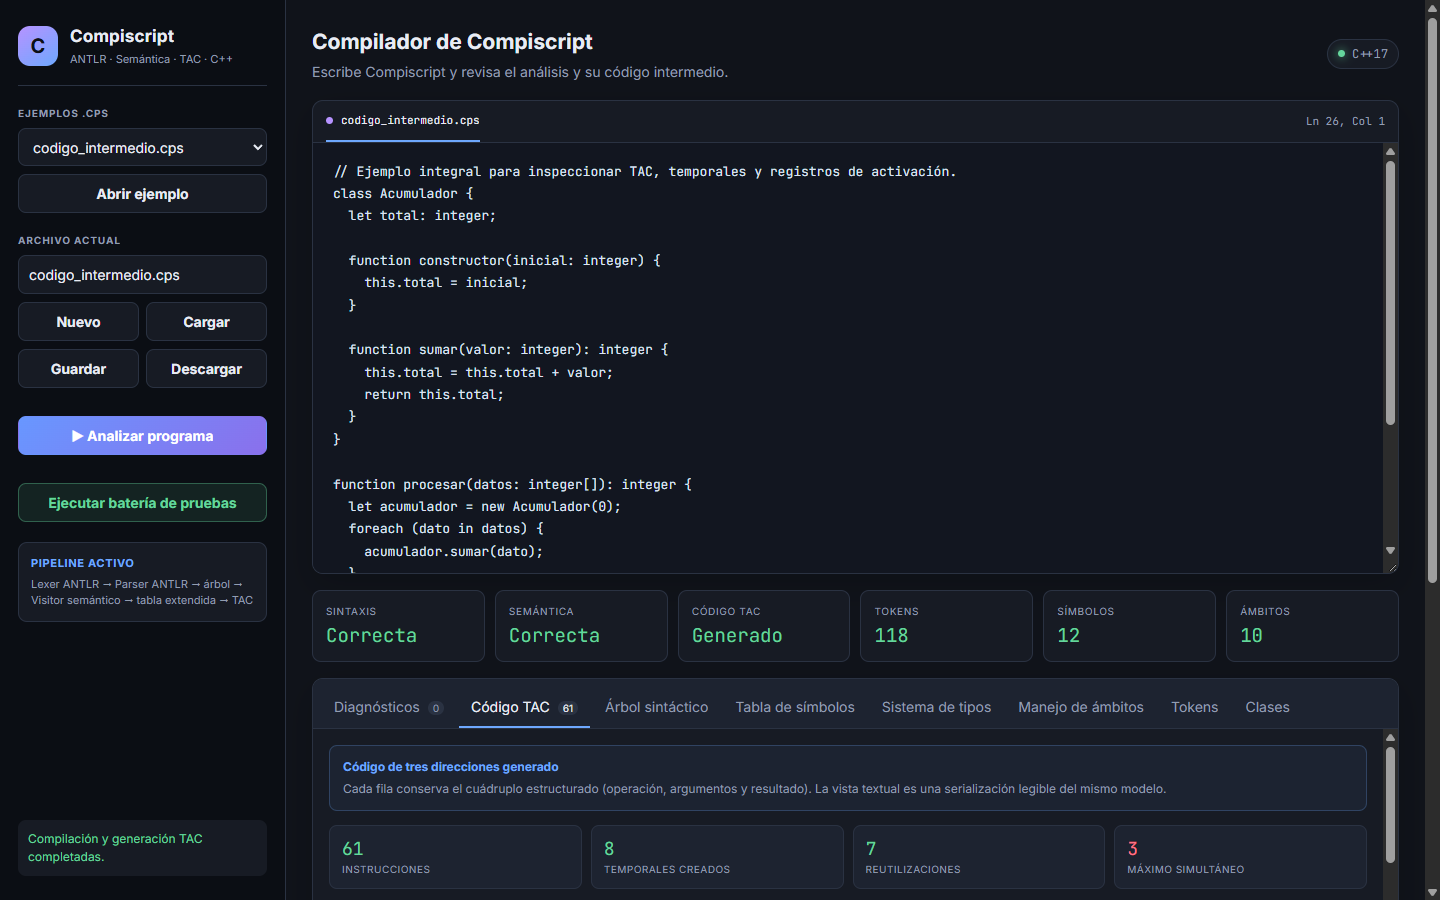
\includegraphics[width=0.9\textwidth]{img/ide-analisis.png}
\caption{Compilación de \texttt{codigo\_intermedio.cps}: sintaxis y semántica
correctas, \emph{Código TAC: Generado}, 118 tokens, 12 símbolos y 10 ámbitos.}
\end{figure}

\subsection{Pestaña Código TAC}

La pestaña muestra primero las métricas del generador (instrucciones,
temporales creados, reutilizaciones y máximo simultáneo) y la representación
textual, con un botón para copiarla.

\begin{figure}[H]
\centering
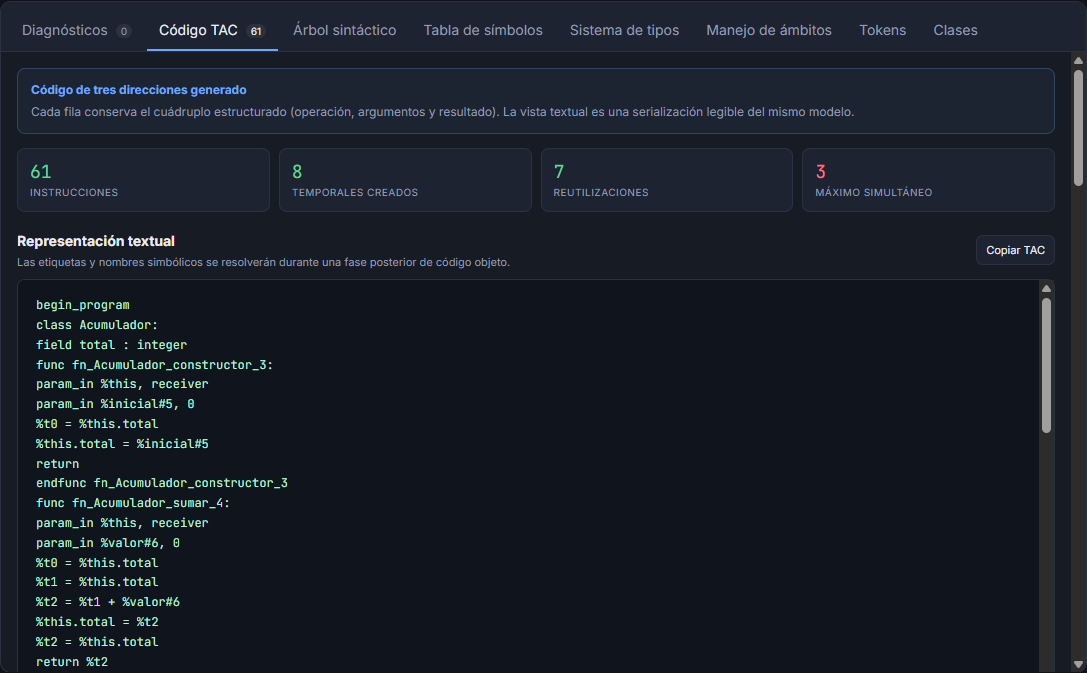
\includegraphics[width=0.96\textwidth]{img/tac-panel-texto.png}
\caption{Métricas y representación textual del TAC de
\texttt{codigo\_intermedio.cps}.}
\end{figure}

Debajo de la vista textual se presenta la tabla de cuádruplos, con la operación,
el resultado, los dos argumentos y la posición de origen (\texttt{línea:columna})
en el archivo fuente. Un guion indica que la forma de instrucción no usa ese
operando.

\begin{figure}[H]
\centering
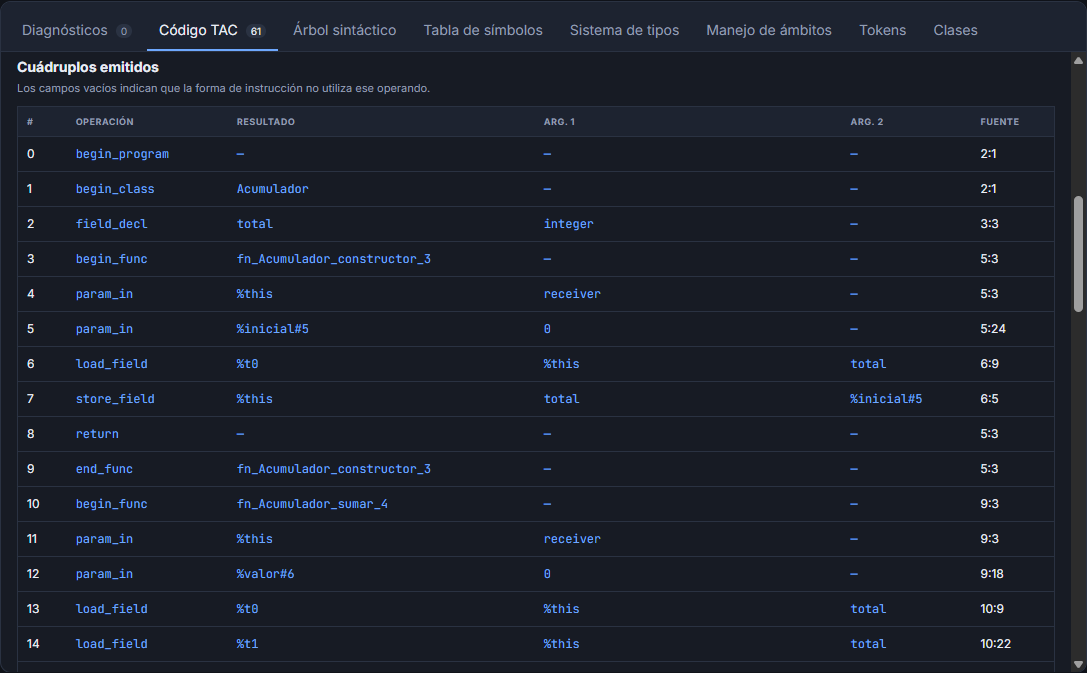
\includegraphics[width=0.96\textwidth]{img/tac-panel-cuadruplos.png}
\caption{Tabla de cuádruplos emitidos.}
\end{figure}

Al final se listan los registros de activación con su etiqueta, profundidad
léxica, bytes de parámetros, locales y temporales, tamaño total y capturas.

\begin{figure}[H]
\centering
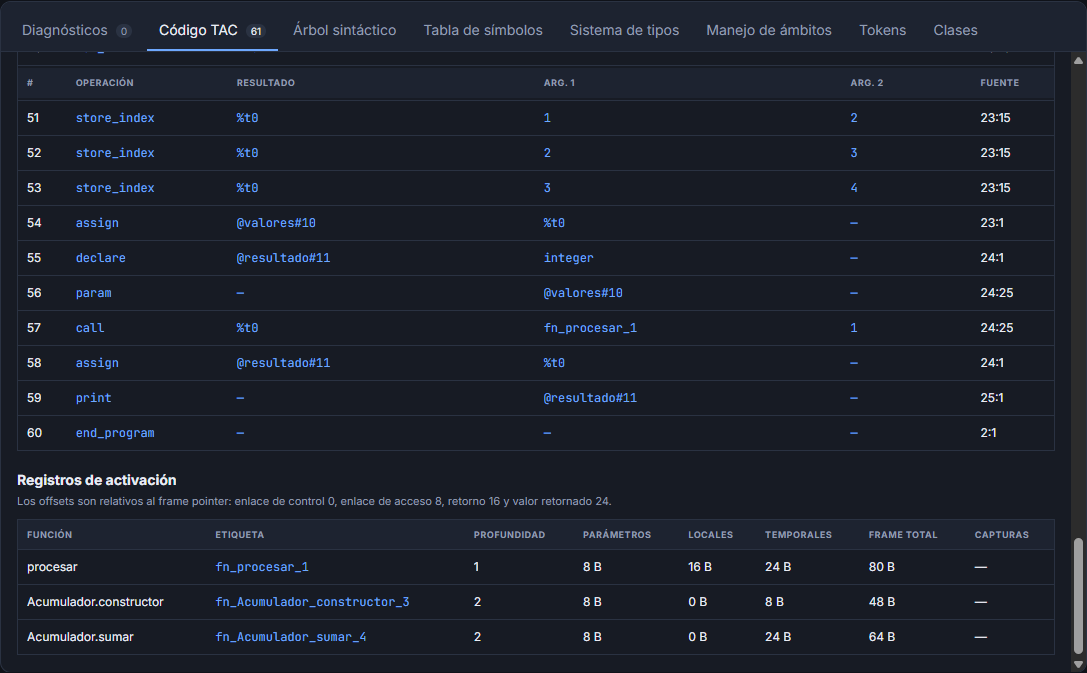
\includegraphics[width=0.96\textwidth]{img/tac-panel-frames.png}
\caption{Últimos cuádruplos y registros de activación de cada función y método.}
\end{figure}

\subsection{Closures en el IDE}

Para \texttt{closures.cps} el TAC incluye \texttt{capture} y \texttt{static\_link},
y el frame de \texttt{sumar} registra la captura de \texttt{base}.

\begin{figure}[H]
\centering
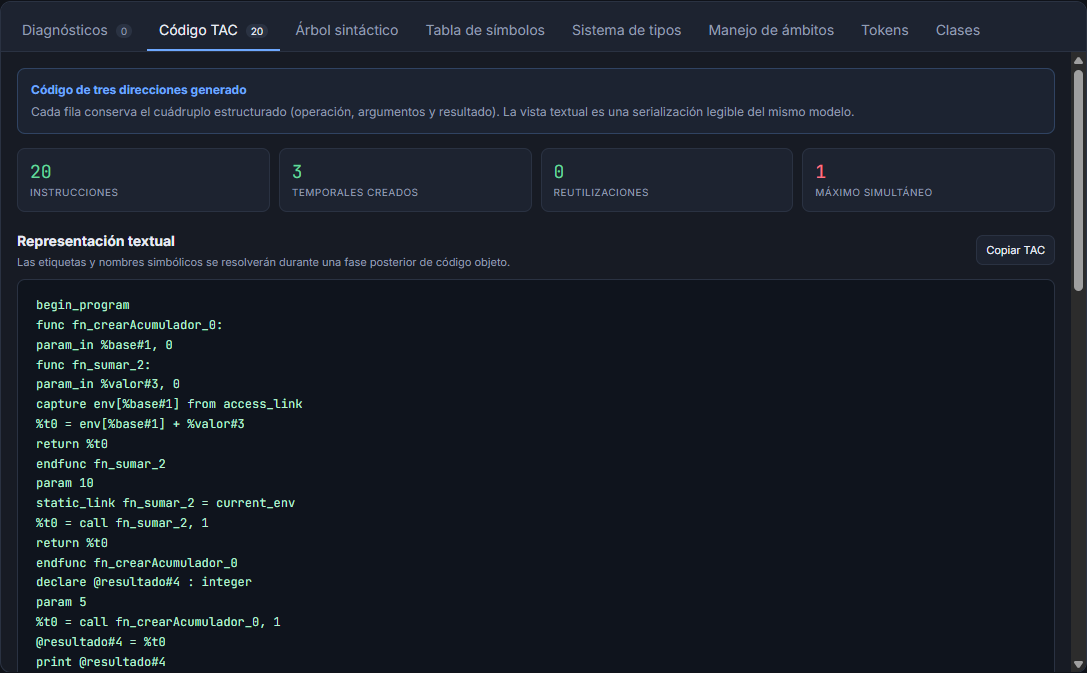
\includegraphics[width=0.96\textwidth]{img/closures-tac-texto.png}
\caption{TAC de \texttt{closures.cps}: \texttt{capture}, acceso \texttt{env[...]}
y \texttt{static\_link}.}
\end{figure}

\begin{figure}[H]
\centering
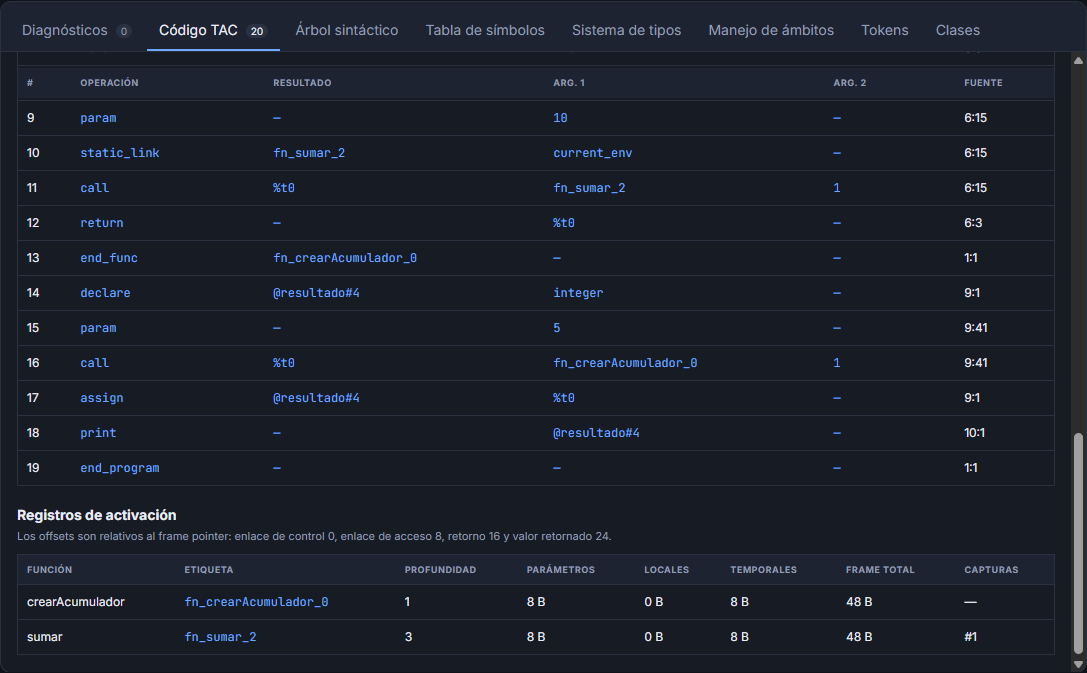
\includegraphics[width=0.96\textwidth]{img/closures-tac-frames.png}
\caption{Frames de \texttt{closures.cps}: \texttt{sumar} (profundidad 3) captura
el símbolo \#1.}
\end{figure}

\subsection{Tabla de símbolos y ámbitos extendidos}

La tabla de símbolos ahora incluye las columnas \emph{Almacenamiento} y
\emph{Offset / tamaño}, y la vista de ámbitos agrega \emph{Profundidad} y
\emph{Frame}.

\begin{figure}[H]
\centering
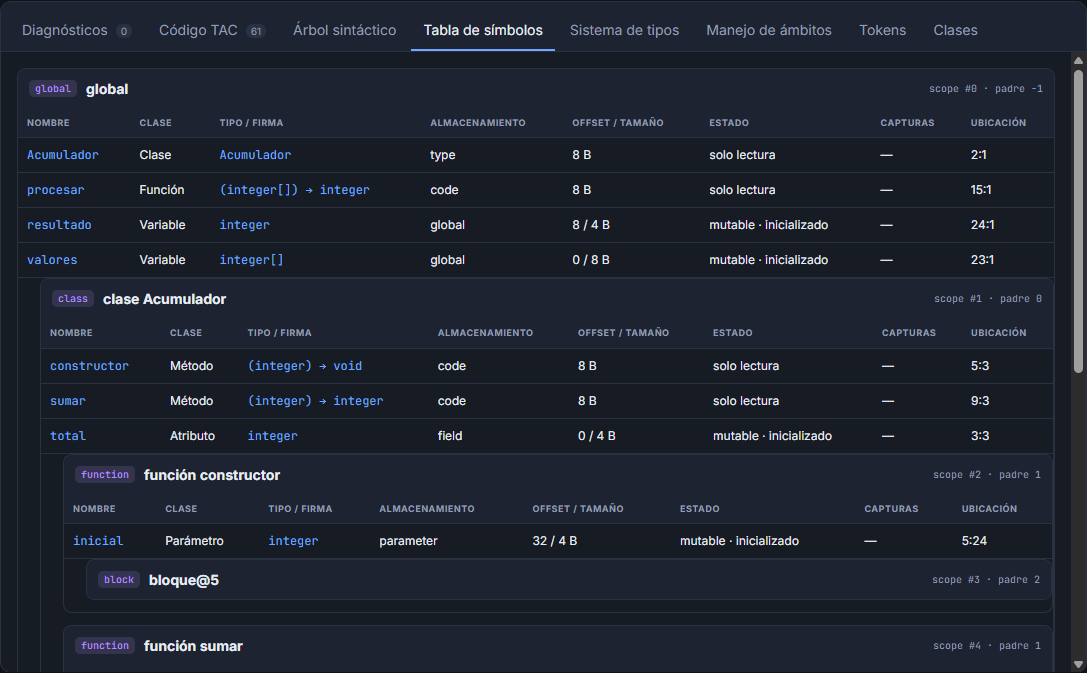
\includegraphics[width=0.96\textwidth]{img/tabla-simbolos-ext.png}
\caption{Tabla de símbolos con almacenamiento, offset y tamaño. \texttt{total}
es un atributo en el offset 0; \texttt{inicial} es un parámetro en el offset 32.}
\end{figure}

\begin{figure}[H]
\centering
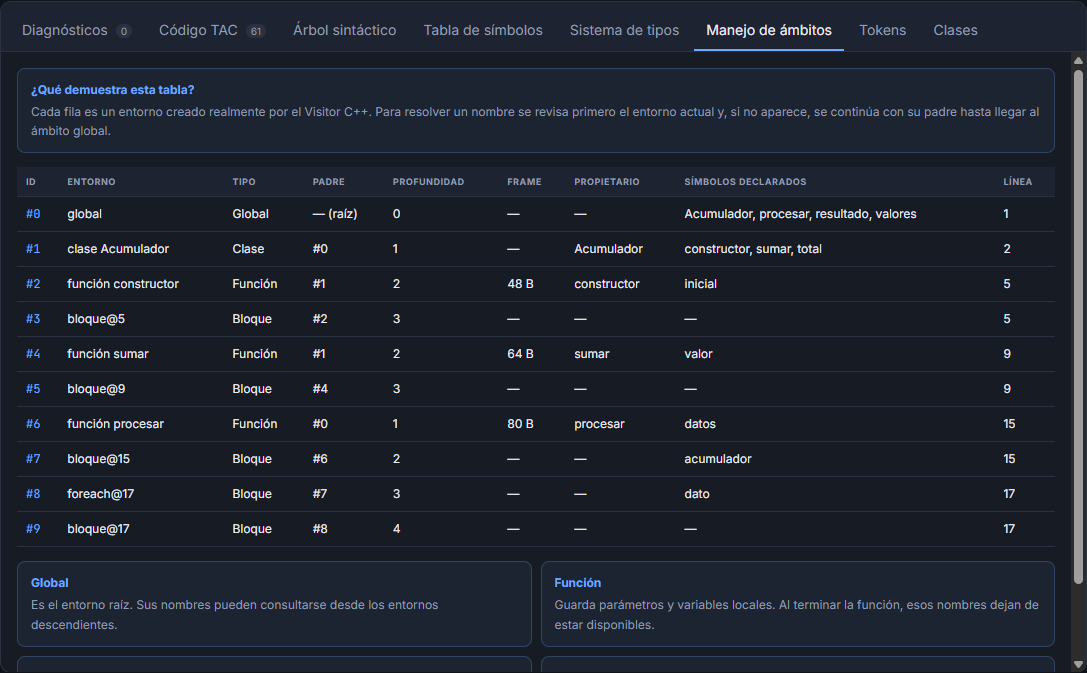
\includegraphics[width=0.96\textwidth]{img/ambitos-ext.png}
\caption{Vista de ámbitos con profundidad léxica y tamaño de frame: 48~B para
el constructor, 64~B para \texttt{sumar} y 80~B para \texttt{procesar}.}
\end{figure}

\subsection{Reporte de errores}

Cuando el programa tiene errores, el IDE sigue mostrando los diagnósticos con su
código, categoría y ubicación, y la tarjeta \emph{Código TAC} indica
\emph{Omitido}. En \texttt{errores\_semanticos.cps} la sintaxis es correcta, la
semántica reporta 17 errores y no se genera código:

\begin{figure}[H]
\centering
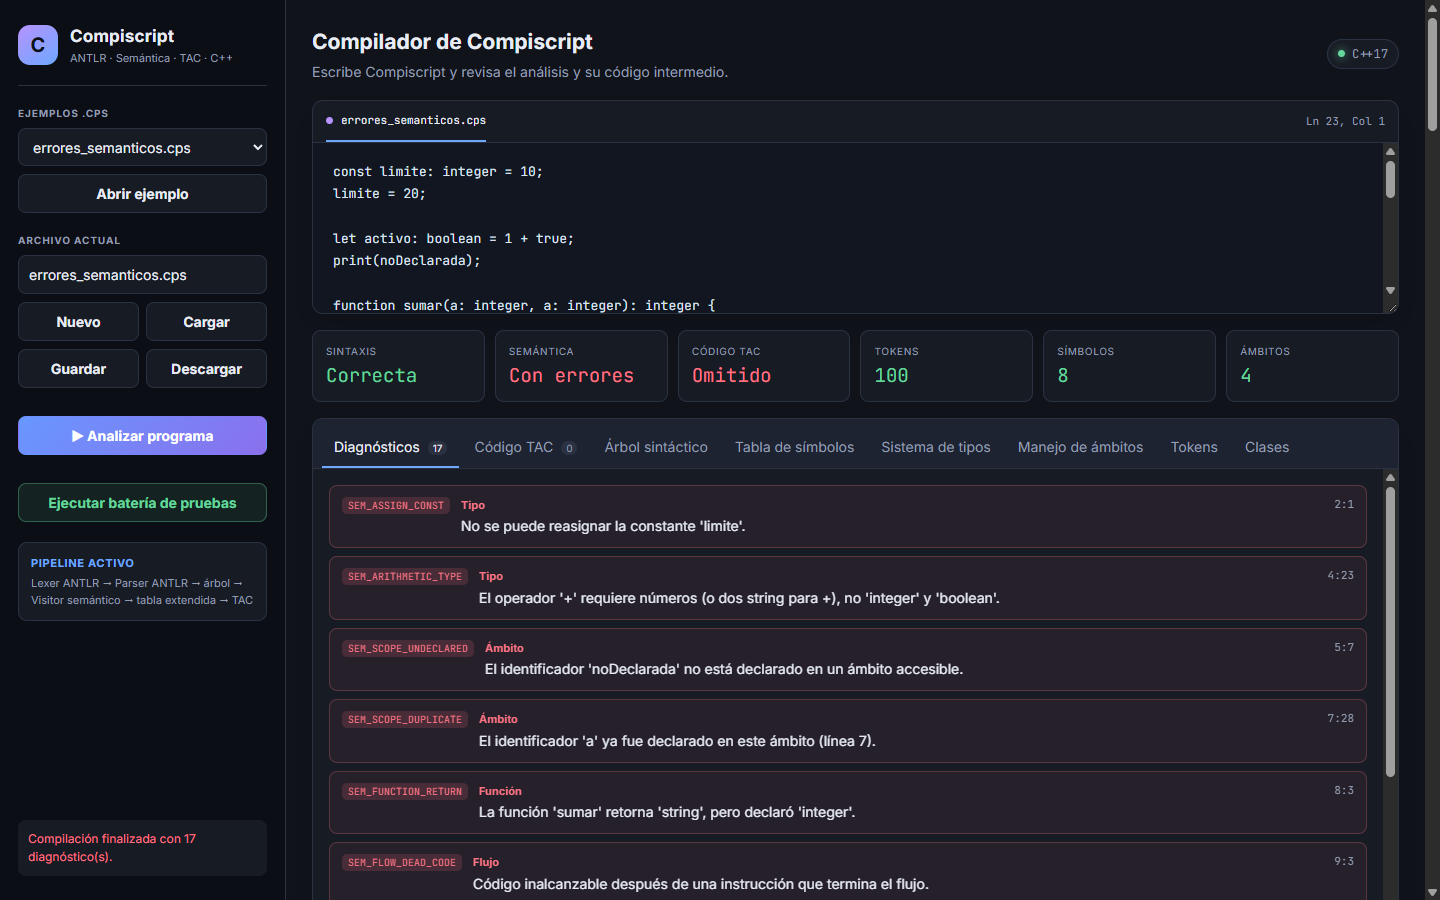
\includegraphics[width=\textwidth]{img/ide-errores.png}
\caption{Compilación de \texttt{errores\_semanticos.cps}: 17 diagnósticos
semánticos y \emph{Código TAC: Omitido}.}
\end{figure}

\begin{figure}[H]
\centering
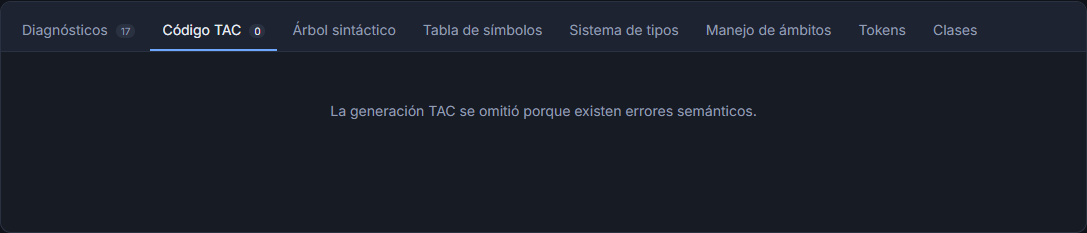
\includegraphics[width=0.96\textwidth]{img/tac-omitido.png}
\caption{La pestaña \emph{Código TAC} explica por qué la generación se omitió.}
\end{figure}

Ante un error sintáctico, tanto la semántica como el TAC se omiten:

\begin{figure}[H]
\centering
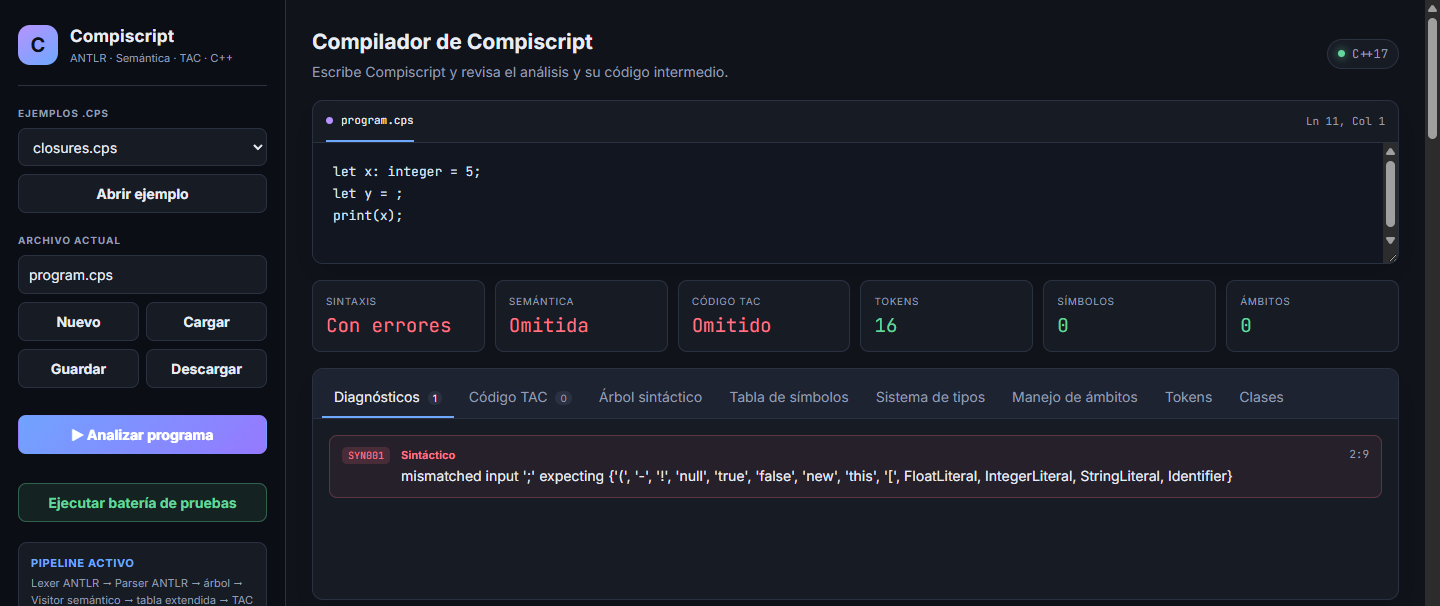
\includegraphics[width=\textwidth]{img/ide-error-sintactico.png}
\caption{Entrada con un error sintáctico (\texttt{let y = ;}): sintaxis con
errores, semántica y TAC omitidos.}
\end{figure}

% ----------------------------------------------------- 11 BATERÍA DE PRUEBAS
\section{Batería de pruebas}

La batería está en \texttt{backend/tests/compiscript\_tests.cpp} y contiene
ahora \textbf{107 escenarios}: 51 programas válidos y 56 errores esperados. Sigue
sin depender de ningún \emph{framework} externo y enlaza directamente contra
\texttt{compiscript\_core}, de modo que prueba el mismo servicio que usan el CLI
y el IDE.

El criterio de un caso negativo sigue siendo estricto: no basta con que el
programa falle, debe fallar \textbf{con el código de diagnóstico correcto}, y en
los casos de TAC además debe quedar marcado como omitido y sin instrucciones.

\begin{table}[H]
\centering
\small
\begin{tabular}{@{}L{6.8cm}rr@{}}
\toprule
\textbf{Categoría} & \textbf{Aprobadas} & \textbf{Total} \\
\midrule
Proceso completo & 4 & 4 \\
Sistema de tipos & 20 & 20 \\
Manejo de ámbito & 7 & 7 \\
Funciones y procedimientos & 13 & 13 \\
Control de flujo & 20 & 20 \\
Clases y objetos & 13 & 13 \\
Listas y estructuras de datos & 11 & 11 \\
Reglas generales & 7 & 7 \\
\textbf{Generación de código intermedio (nueva)} & \textbf{12} & \textbf{12} \\
\midrule
\textbf{Total} & \textbf{107} & \textbf{107} \\
\bottomrule
\end{tabular}
\caption{Resultado de la batería por categoría.}
\end{table}

\subsection{Escenarios de generación de código}

\begin{table}[H]
\centering
\small
\begin{tabular}{@{}L{3.4cm}L{3.4cm}L{7.4cm}@{}}
\toprule
\textbf{Tema} & \textbf{Entrada} & \textbf{Qué verifica} \\
\midrule
Precedencia & \texttt{2 + 3 * 4} & \texttt{mul} se emite antes que \texttt{add}
y no hay diagnósticos. \\
Cortocircuito & \texttt{(true \&\& false) || true} & Hay \texttt{if\_true},
\texttt{if\_false} y etiquetas. \\
Control de flujo & \texttt{for} con \texttt{continue} y \texttt{break} & Al
menos 3 \texttt{goto} y 5 etiquetas. \\
\texttt{switch} & selector booleano con dos \texttt{case} & Exactamente dos
comparaciones \texttt{eq}; sin caída. \\
Funciones & \texttt{factorial} recursivo & \texttt{begin\_func},
\texttt{param\_in}, \texttt{call}, \texttt{return} y frame no vacío. \\
Closures & función anidada que usa \texttt{base} & Frame con símbolos
capturados, \texttt{capture} y \texttt{static\_link}. \\
Clases & constructor, campo y método & \texttt{new\_object},
\texttt{load\_field}, \texttt{store\_field} y \texttt{call\_method}. \\
Listas & creación, lectura y escritura & \texttt{new\_list},
\texttt{load\_index} y \texttt{store\_index}. \\
Temporales & tres sumas encadenadas & Se reutiliza al menos un temporal ya
consumido. \\
Tabla extendida & globales, parámetros y locales & Todo símbolo con valor tiene
\texttt{storage} y \texttt{offset}; el frame trae parámetros y locales y mide
al menos 32 B. \\
Omisión semántica & \texttt{let x: integer = true;} & \texttt{SEM\_ASSIGN\_TYPE},
TAC omitido y sin instrucciones. \\
Omisión sintáctica & \texttt{let x = ;} & Semántica y TAC omitidos y sin
instrucciones. \\
\bottomrule
\end{tabular}
\caption{Los 12 escenarios agregados en el commit \texttt{66f83c3}.}
\end{table}

\begin{figure}[H]
\centering
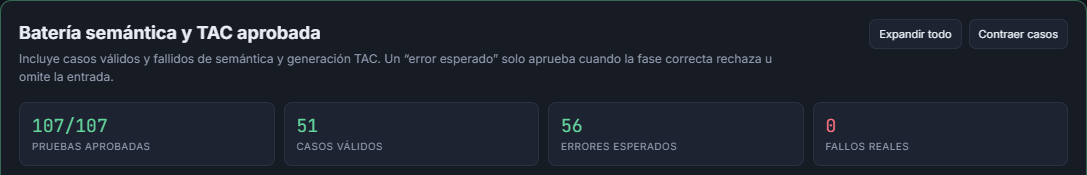
\includegraphics[width=\textwidth]{img/pruebas-resumen.png}
\caption{Batería ejecutada desde el IDE: 107/107 aprobadas, 51 casos válidos,
56 errores esperados y 0 fallos reales.}
\end{figure}

\begin{figure}[H]
\centering
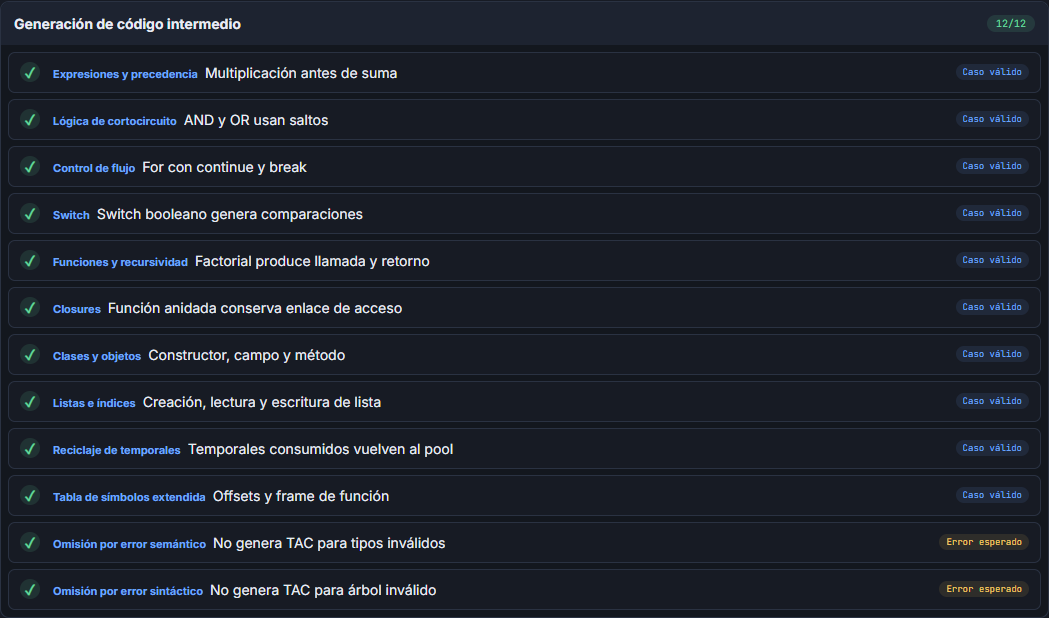
\includegraphics[width=0.96\textwidth]{img/pruebas-tac.png}
\caption{Categoría \emph{Generación de código intermedio}: 12/12.}
\end{figure}

La batería también puede ejecutarse desde la línea de comandos:

\begin{lstlisting}[language=bash,caption={Ejecución desde CTest.}]
ctest --test-dir build/compiscript --output-on-failure
\end{lstlisting}

% ------------------------------------------------ 12 COMPILACIÓN Y EJECUCIÓN
\section{Compilación y ejecución}

\subsection{Requisitos}

\begin{itemize}[leftmargin=1.4em]
  \item CMake 3.20 o superior.
  \item Compilador compatible con C++17.
  \item Java, únicamente para ejecutar la herramienta generadora de ANTLR (el
        código generado ya está versionado en el repositorio).
  \item Python 3 con Flask, únicamente para servir el IDE.
\end{itemize}

\subsection{Construcción}

Un solo script descarga el JAR oficial de ANTLR si hace falta, regenera el lexer,
el parser y el Visitor, descarga y compila el \emph{runtime} C++ de ANTLR,
construye \texttt{compiscript\_cli} y \texttt{compiscript\_tests}, y ejecuta la
batería:

\begin{lstlisting}[language=bash,caption={macOS o Linux.}]
python3 -m pip install -r requirements.txt
./scripts/build_compiscript.sh
\end{lstlisting}

\begin{lstlisting}[language=bash,caption={Windows PowerShell.}]
python -m pip install -r requirements.txt
powershell -File scripts/build_compiscript.ps1
\end{lstlisting}

\subsection{Ejecución del IDE}

\begin{lstlisting}[language=bash,caption={Servidor del IDE.}]
python app.py
\end{lstlisting}

El IDE queda disponible en \texttt{http://127.0.0.1:5050}. Se abre un ejemplo,
se pulsa \emph{Analizar programa} y se selecciona la pestaña \emph{Código TAC}.

\subsection{Uso directo del CLI}

\begin{lstlisting}[language=bash,caption={Compilación desde la línea de comandos.}]
./compiscript_cli --file backend/examples/compiscript/codigo_intermedio.cps
./compiscript_cli --stdin program.cps < program.cps
\end{lstlisting}

La salida es un único documento JSON con los bloques \texttt{tokens},
\texttt{tree}, \texttt{semantic} y \texttt{tac} (\texttt{text},
\texttt{instructions}, \texttt{activation\_records}, \texttt{temporaries\_*}).
El código de salida es 0 cuando no hay errores, 1 cuando el programa contiene
diagnósticos y 2 cuando el uso del CLI o el archivo de entrada no son válidos.

\subsection{Verificación realizada para este informe}

Para escribir este informe se compiló y probó la rama
\texttt{Compiladores2-Proyecto2} en Windows 11 con GCC 14.2 (MinGW-w64), CMake
3.31 y Ninja, usando el código fuente del \emph{runtime} de ANTLR 4.13.2 ya
disponible localmente. Los resultados observados fueron:

\begin{itemize}[leftmargin=1.4em]
  \item La construcción completó sus 154 pasos sin errores.
  \item \texttt{compiscript\_tests}: \textbf{107/107 pruebas aprobadas}; CTest
        reportó 1 de 1 pruebas superadas.
  \item \texttt{compiscript\_cli} sobre \texttt{codigo\_intermedio.cps} terminó
        con código 0 y generó 61 instrucciones; sobre
        \texttt{errores\_semanticos.cps} terminó con código 1.
  \item El IDE respondió en \texttt{http://127.0.0.1:5050} y todas las capturas
        de este documento provienen de esa ejecución.
\end{itemize}

% ----------------------------------------------- 13 DECISIONES Y SUPUESTOS
\section{Decisiones, supuestos y limitaciones}

Las decisiones siguientes están documentadas en el repositorio y son las que un
calificador necesita para interpretar el TAC.

\begin{itemize}[leftmargin=1.4em]
  \item \textbf{Solo se genera TAC para programas válidos.} Léxico, sintaxis y
        semántica deben terminar sin errores; si no, el TAC se marca como
        omitido y no hay instrucciones.
  \item \textbf{Las etiquetas son simbólicas.} Todavía no son direcciones de
        máquina; su resolución corresponde a la fase de código objeto.
  \item \textbf{\texttt{switch} no tiene caída implícita.} Cada \texttt{case}
        salta al final, coherente con la regla del proyecto que reserva
        \texttt{break} para ciclos.
  \item \textbf{Orden de evaluación.} Los argumentos se evalúan de izquierda a
        derecha y \texttt{\%this} se pasa antes de los argumentos explícitos de
        un método.
  \item \textbf{Las listas son referencias dinámicas.} \texttt{foreach} se baja a
        índice, \texttt{length}, comparación, lectura y salto.
  \item \textbf{\texttt{try/catch} se conserva con operaciones abstractas}
        porque el proyecto no define un ABI de excepciones.
  \item \textbf{El TAC es una representación intermedia, no un intérprete ni
        código objeto.} No se ejecuta; su corrección se valida estructuralmente
        con la batería de pruebas.
  \item \textbf{Frames abstractos.} Los tamaños (1, 4, 8 bytes) y la alineación
        a 8 bytes son supuestos del modelo, no de una arquitectura concreta.
\end{itemize}

\paragraph{Limitaciones conocidas.}

\begin{itemize}[leftmargin=1.4em]
  \item No hay optimización: no se pliegan constantes (\texttt{1 + 2} genera una
        suma), no se elimina código muerto del TAC y no hay asignación de
        registros.
  \item En una asignación a un atributo o a un elemento de lista, el generador
        carga primero el lado izquierdo para conservar su localización, lo que
        deja una lectura cuyo valor no se usa (por ejemplo,
        \texttt{\%t0 = \%this.total} antes de \texttt{\%this.total = \dots}).
  \item Las verificaciones de la batería son estructurales (presencia y orden de
        operaciones, métricas, \emph{layout}); no se interpreta el TAC para
        comparar resultados de ejecución.
\end{itemize}

% --------------------------------------------------- 14 RÚBRICA
\section{Correspondencia con la rúbrica}

\begin{table}[H]
\centering
\small
\begin{tabular}{@{}L{3.6cm}rL{9.4cm}@{}}
\toprule
\textbf{Componente} & \textbf{Pts} & \textbf{Evidencia en el proyecto} \\
\midrule
Diseño de CI & 25 &
Lenguaje de cuádruplos con formas de dirección, conjunto de instrucciones y
sintaxis textual (sección~6), ejemplos de traducción por construcción
(sección~7) y supuestos (sección~13); documentado también en
\texttt{docs/codigo-intermedio-tac.md}. \\
Generación de TAC & 65 &
\texttt{TacGenerator} de 1\,211 líneas: expresiones, control de flujo,
funciones, recursión, closures, clases, objetos y listas; reciclaje de
temporales (sección~8); batería de 107 escenarios con 12 específicos de TAC
(sección~11). \\
Tabla de símbolos & 10 &
Campos \texttt{size}, \texttt{offset}, \texttt{storage},
\texttt{lexical\_depth} y \texttt{label}; registros de activación con enlaces de
control y acceso, retorno, parámetros, locales y temporales (sección~9);
visibles en el IDE. \\
\midrule
\textbf{Total} & \textbf{100} & \\
\bottomrule
\end{tabular}
\caption{Evidencia por componente evaluado.}
\end{table}

Respecto a los entregables: el repositorio conserva commits individuales por
integrante (sección~4), la batería cubre casos exitosos y fallidos de la
generación de código (sección~11), la arquitectura y las instrucciones de
ejecución están documentadas (secciones~3 y 12, además de
\texttt{docs/arquitectura-compiscript.md} y \texttt{README.md}), el lenguaje
intermedio tiene su documento propio y el IDE es funcional (sección~10).

% ---------------------------------------------------- 15 CONCLUSIONES
\section{Conclusiones}

\begin{enumerate}[leftmargin=1.6em]
  \item Separar el análisis semántico y la generación de código en dos Visitors
        evitó duplicar la resolución de nombres: el puente
        \texttt{SemanticBindings} permite que el generador trabaje con
        identificadores de símbolo en lugar de texto.
  \item Generar TAC solo para programas sin errores simplifica el generador y
        elimina la posibilidad de producir código parcial o engañoso para
        entradas inválidas; el IDE y la batería lo verifican explícitamente.
  \item El pool de temporales por función demuestra que el número de temporales
        necesarios depende del máximo de valores simultáneamente vivos y no del
        tamaño del programa: el ejemplo integral usa 8 temporales creados y 7
        reutilizaciones, con a lo sumo 3 vivos a la vez.
  \item Extender la tabla de símbolos con tamaños, offsets y frames, en lugar de
        crear una estructura aparte, mantiene una única fuente de verdad que el
        IDE, las pruebas y las fases posteriores pueden consultar.
  \item Las limitaciones identificadas (sin optimización, lectura redundante del
        lado izquierdo, TAC no ejecutable) delimitan con claridad qué
        corresponde a las fases siguientes: optimización y generación de código
        objeto.
\end{enumerate}

% ---------------------------------------------------- 16 REFERENCIAS
\section{Referencias}

\begin{itemize}[leftmargin=1.4em]
  \item Aho, A., Lam, M., Sethi, R. y Ullman, J. \emph{Compilers: Principles,
        Techniques, and Tools}. 2.\textordfeminine{} edición, 2006. Capítulo 6
        (código intermedio, cuádruplos y traducción dirigida por sintaxis) y
        secciones 7.2 y 7.3 (registros de activación y acceso a datos no
        locales).
  \item Parr, T. \emph{The Definitive ANTLR 4 Reference}. Documentación del
        \emph{target} de C++: \url{https://github.com/antlr/antlr4}.
  \item Enunciado del proyecto: \emph{Proyecto 2: Generación de Código
        Intermedio para Compiscript}, Construcción de Compiladores, septiembre
        de 2026.
  \item Repositorio del proyecto, rama \texttt{Compiladores2-Proyecto2}:
        \url{https://github.com/G1LB3T0/Proyecto1_Compis_Generador_Analizador_Lexico}.
  \item Documentación interna del repositorio, en la carpeta \texttt{docs/}:
        \texttt{codigo-intermedio-tac.md}, \\
        \texttt{arquitectura-compiscript.md} y
        \texttt{decisiones-compiscript.md}.
\end{itemize}

\end{document}
